
\documentclass{article}
\usepackage[spanish]{babel}
\usepackage[utf8]{inputenc}
\usepackage{graphicx}
\usepackage{float}
%\usepackage{subfig}
\usepackage{xcolor}
\usepackage{hyperref}
\usepackage{pythonhighlight}
\usepackage[margin=1 in]{geometry}%medida de los margenes
\usepackage{wrapfig}
\usepackage{tikz}
\usepackage{setspace}
\usepackage{mathtools}
\usepackage{tcolorbox}
\usepackage{amsfonts}
\usepackage{amssymb}
\usepackage{subcaption}
\tcbuselibrary{listings,theorems}
%\noindent para quitar el sangrado
%La opción pages puede ser all (para todo el documento) o some, para algunas partes del documento
\usepackage[pages=some]{background}
% configuración
\backgroundsetup{
 scale=1, %escala de la imagen, es recomendable que sea del mismo tamaño que el pdf
 color=black, %fondo a usar para transparencia
 opacity=0.7, %nivel de transparencia
 angle=0, %en caso de querer una rotación
 contents={%
  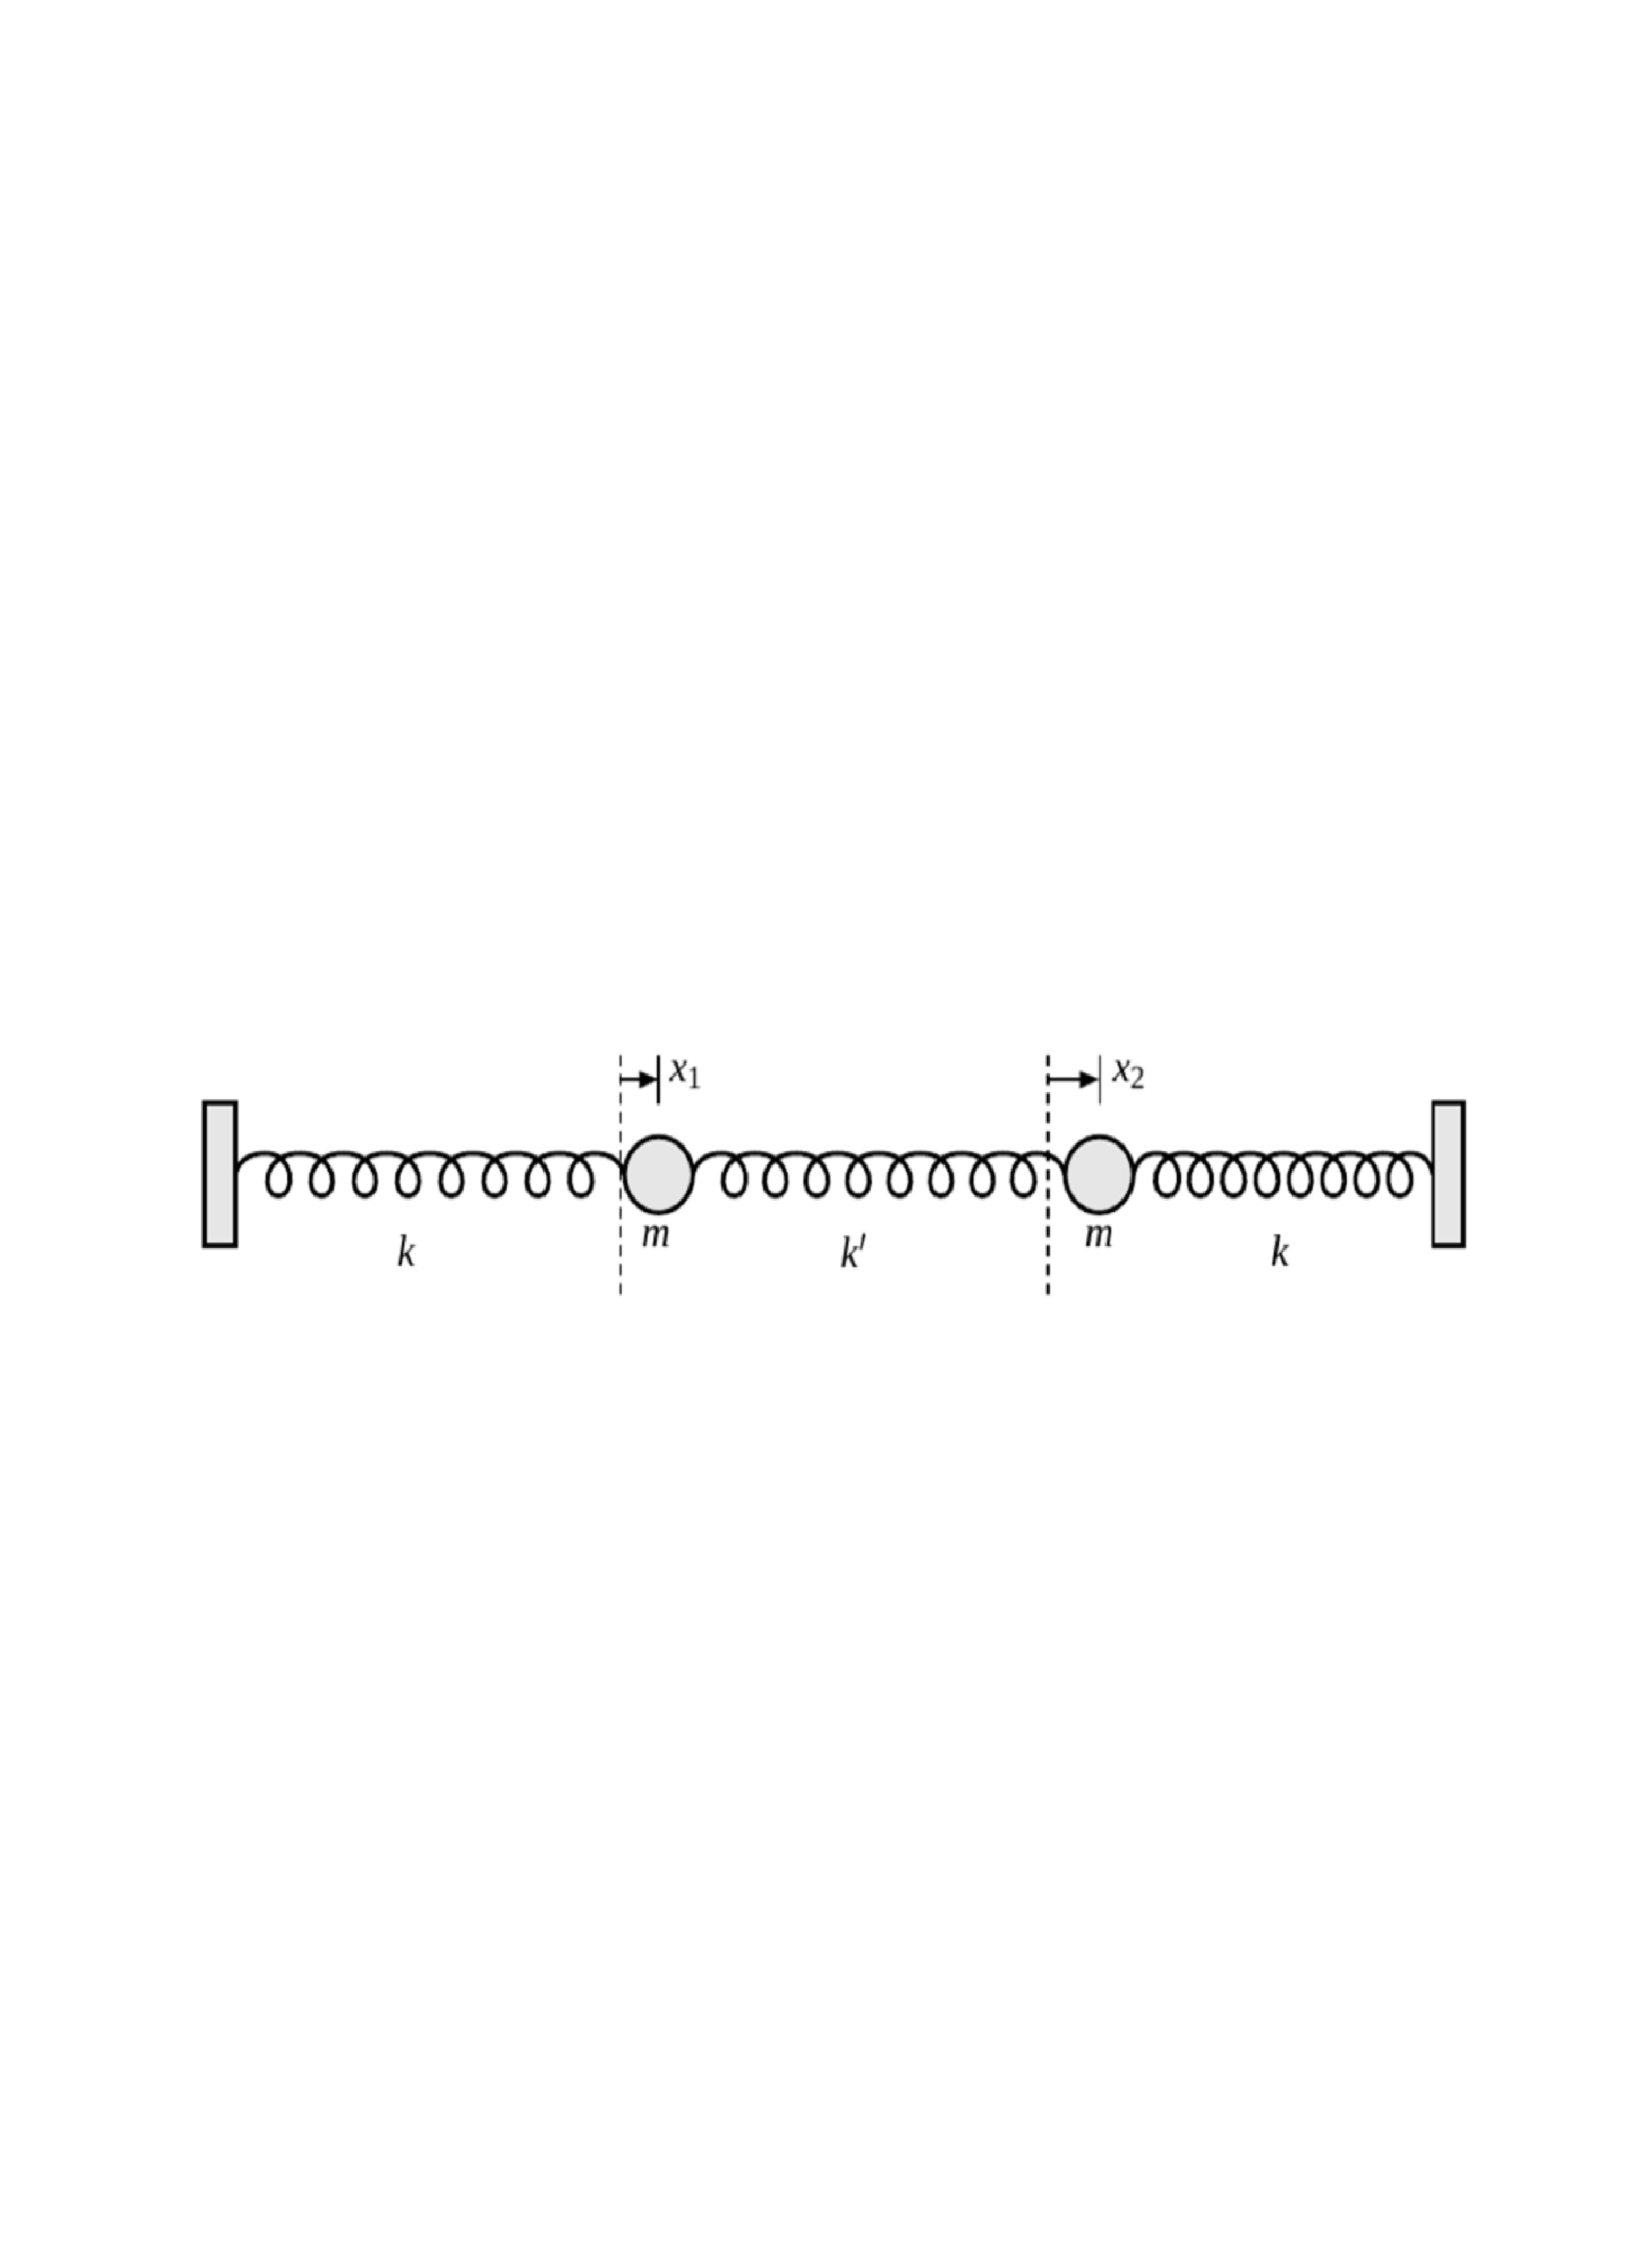
\includegraphics[width=\paperwidth,height=\paperheight]{port} %nombre de la imagen a utilizar como fondo
 }%
}
%definimos colores:
\definecolor{azul}{RGB}{0,160,255}
\definecolor{azul2}{RGB}{7,74,163}
\definecolor{blanco}{RGB}{250,250,250}
\definecolor{amarillo}{RGB}{252,250,129}
%Cuerpo
\begin{document}

\definecolor{w}{rgb}{255,255,255}
\hypersetup{linkbordercolor={w},urlbordercolor={w},citebordercolor={0 0 0}}


\BgThispage 
\begin{titlepage}
	\thispagestyle{empty} % No header nor footer
	%\newgeometry{left=2cm,right=1cm, top=2cm, bottom=2cm}
	\begin{tikzpicture}[overlay,fill opacity=0.7]	
		%\rotatebox{0}{\fill[amarillo] (-1,-1) rectangle (16.5,-5);}
		%\rotatebox{0}{\fill[blanco] (2,-6.5) rectangle (15.5,-17);}
	\end{tikzpicture}

{\itshape\Large \par}
\vspace{1.75cm}
\centering
{\scshape\Huge Práctica 2\par}
{\scshape\Huge Osciladores acoplados \par}
%{\scshape\Huge Circuitos rlc en serie. Resonancia\par}
\vspace{3cm}
\centering
%{
\includegraphics[width=0.65\textwidth]{portada}\par}
\vfill
\vspace{10cm}
{\Large Autora: \par}
{\Large Aroa Antón Samaniego \par}
\vfill
{\itshape\Large Mecánica analítica. Prácticas de ordenador. Grado en Física. \par}
{\centering\Large Curso 2022-2023 \par}
\end{titlepage}
    \tableofcontents\hspace{5cm}\pagebreak
\section{Introducción}
En esta práctica vamos a estudiar el movimiento de un oscilador de muelles acoplados. Para ello vamos a simular el movimiento del sistema mediante un programa de Python. También estudiaremos sus modos normales de vibración, que nos permitirán observar casos como el modo de vibración simmétrico y antisimétrico. 
\section{Fundamento teórico}
Tenemos un sistema compuesto por dos masas $m_1$ y $m_2$ unidas a una pared por un muelle de constante elástica $k$ y a su vez unidas entre si por otro muelle de constante $k'$ como podemos ver en la figura:
\begin{figure}[H]
    \centering
    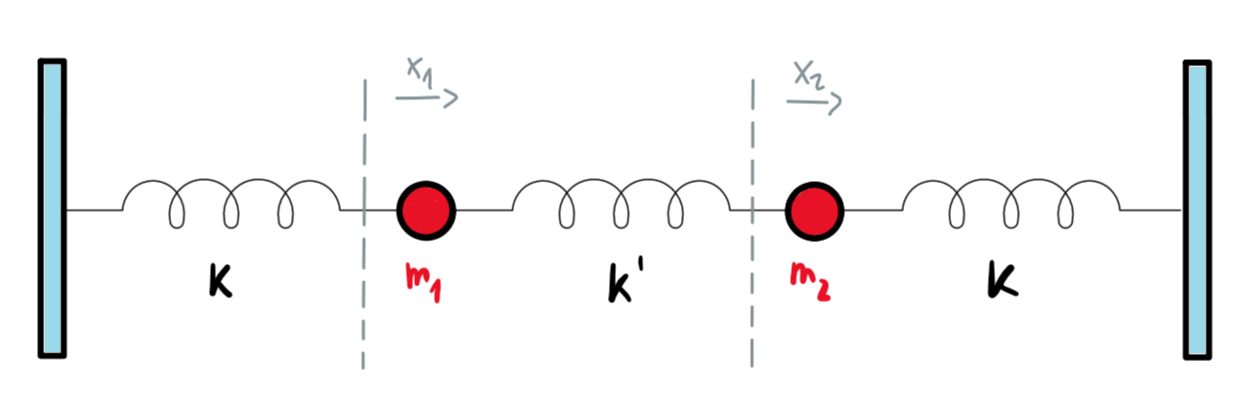
\includegraphics[width=0.8\textwidth]{muelles}
%\caption{Diagrama del sistema}
\label{fig:0}
\end{figure}
\noindent Vamos a considerar que nuestras masas solo se van a mover en una dimensión por lo que nuestro sistema va a tener dos grados de libertad y nuestras variables van a ser las posiciones de la masas $m_1$ y $m_2$ que daremos con las coordenadas $x_1$ y $x_2$ tomando como origen la pared más cercana a la masa $m_1$.\newline\linebreak
Las fuerzas que actuarán sobre cada masa serán:\vspace{0.3cm}
\begin{itemize}
\item $Masa\hspace{0.2cm} m_1 \rightarrow F_1 = -kx_1 -k'(x_1-x_2)$
\item $Masa\hspace{0.2cm} m_2 \rightarrow F_2 = -kx_2 -k'(x_2-x_1)$
\end{itemize}\vspace{0.3cm}
Suponiendo que el valor de ambas masas va a ser el mismo ($m_1 = m_2 = m$) y gracias a la 2ª Ley de Newton ($\sum F = ma$) podemos plantear las ecuaciones de movimiento del sistema:

\begin{equation}
m\ddot{x_1}+(k+k')x_1 -k'x_2  = 0\label{ec.:1}
\end{equation}
\begin{equation}
m\ddot{x_2}+(k+k')x_2 -k'x_1  = 0\label{ec.:2}
\end{equation}
Podemos proponer soluciones oscilatorias a estas ecuaciones de la forma:
\begin{equation}\left.
x_1(t)=B_1e^{iwt}\atop
x_2(t)=B_2e^{iwt}
\right\}\end{equation}
Para que estas expresiones sean solución de las ecuaciones obtenemos que se debe cumplir:
\begin{equation}
\omega = \sqrt{\frac{k+k'\pm k'}{m}}
\end{equation}
Por lo tanto vamos a tener dos pulsaciones propias del sistema, que tendrán frecuencias de pulsación características:\newline
\begin{equation}\tcboxmath[colback=blue!10!white,colframe=blue!25!white]{\omega_1 = \sqrt{\frac{k+2k'}{m}}\hspace{2cm}\omega_2 = \sqrt{\frac{k}{m}}}\label{ec.:5}\end{equation}
\subsection{Modos normales}
Para simplificar la resolución del problema vamos a hacer un cambio de coordenadas del sistema y vamos a hallar los modos normales, que van a ser las frecuencias de oscilación de cada una de las partes del sistema, consiguiendo así ecuaciones que no van a estar acopladas ,como sí lo estan las ecuaciones (\ref{ec.:1}) y (\ref{ec.:2}).\newline\linebreak
Haciendo el siguiente cambio de coordenadas:
\begin{equation}\notag\left.
\eta_1 = x_1+x_2\atop
\eta_2 = x_1-x_2
\right\}\end{equation}
Llegamos a las nuevas ecuaciones de movimiento:

\begin{equation}\left.
m\ddot{\eta_1} + (k+2k')\eta_1 = 0\atop
m\ddot{\eta_2} + k\eta_2 = 0
\right\}\end{equation}
Cada una de estas ecuaciones corresponderá a un movimiento armónico con frecuencia $\omega_1$ u $\omega_2$. Dándole ciertas condiciones iniciales a nuestro sistema podemos  obtener distintos modos de oscilación.\newline\linebreak
Tomando como condiciones iniciales $x_1(0)=x_2(0)$ y $\dot{x_1}(0)=\dot{x_2}(0)$ tendremos que $\eta_1(t) = 0 \forall t$. Por lo tanto, ambas masas oscilarán con frecuencia $\omega_2$ y en fase. A esta manera de oscilar la conocemos como \textbf{modo normal simétrico de oscilación}.\newline\linebreak
También podemos hacer que las masas oscilen en oposición de fase con una frecuencia de $\omega_1$ considerando como condiciones iniciales $x_1(0)=-x_2(0)$ y $\dot{x_1}(0)=-\dot{x_2}(0)$. En este caso $\eta_1(t) = 0 \forall t$ y decimos que las masas están oscilando en el \textbf{modo normal antisimétrico}.\newline\linebreak
Además, vamos a poder describir el movimiento de cada masa como combinación lineal de estos modos normales:
\begin{equation}
x_1(t) = A_0^1sen(\omega_1t+\phi_1)+A_0^2sen(\omega_2t+\phi_2)
\end{equation}
\begin{equation}
x_1(t) = A_0^1sen(\omega_1t+\phi_1)-A_0^2sen(\omega_2t+\phi_2)
\end{equation}
Si consideramos que $k'\lll k$ se va a dar un caso particular llamado \textbf{acoplamiento débil}. En este caso como la constante elástica del muelle que une ambas masas es mucho menor que la de los muelles que unen estas a las paredes las masas van a estar ligadas débilmente en comparación a las fuerzas que las ligan a las paredes.\newline\linebreak
Esto da lugar a que las dos frecuencias normales de oscilación sean muy parecidas entre ellas y parecidas a la frecuencia natural de uno de los osciladores si dejáramos el otro quieto. Por ello obtenemos un tipo de movimiento que se conoce como latido o pulsos de batido que viene descrito por las ecuaciones:
\begin{equation}x_1(t)=\left(A_0cos(\omega_0 t\varepsilon)\right)cos\omega_0t\label{ec.:9}\end{equation}
\begin{equation}x_2(t)=\left(A_0sen(\omega_0 t\varepsilon)\right)sen\omega_0t\label{ec.:10}\end{equation},donde $\omega_0=\sqrt{\frac{k+k'}{m}}$ es la frecuencia natural de uno de los osciladores si ignoramos el otro y $\varepsilon = \frac{k'}{2k}\lll 1$.\newline\linebreak
\subsection{Transformada de Fourier}
La Transformada de Fourier es una herramienta matemática que se utiliza para analizar señales y descomponerlas en sus componentes de frecuencia. Fue desarrollada por el matemático francés Jean-Baptiste Joseph Fourier en el siglo XIX.\newline\linebreak
En nuestro caso vamos a utilizar la Transformada rápida de Fourier (FFT) que es una manera de hallar fácilmente la Transformada de Fourier para sistemas discretos. Esto nos va a permitir hallar las frecuencias naturales del sistema y cómo se afectan mutuamente debido al acoplamiento, ya que cada oscilador tiene su frecuencia natural propia pero el acoplamiento de los osciladores puede modificar estas.\newline\linebreak
Ahora que ya estamos en contexto vamos a analizar los resultados de la simulación que hemos hecho de nuestro sistema para ver si se comporta como hemos predicho.
\section{Dinámica del sistema}
En este apartado vamos a observar los distintos tipos de movimiento que tiene el sistema para distintos valores de la constante elástica ($k'$) del muelle que une las masas.\newline\linebreak Consideraremos los siguientes datos:
\begin{itemize}
\item $m = 1\hspace{0.1cm}kg$
\item $k = 10 \hspace{0.1cm}N/m$
\item Posición de equilibrio de la masa 1: $x_1 = 1 \hspace{0.1cm}m$
\item Posición de equilibrio de la masa 2: $x_2 = 2 \hspace{0.1cm}m$
\item $x_1 (0)= 0.1 \hspace{0.1cm}m$
\item $x_2 (0)= 0 \hspace{0.1cm}m$
\item $\dot{x_1 }(0)=\dot{x_2}(0)= 0\hspace{0.1cm}m/s$
\end{itemize}
Además, también será interesante observar el comportamiento de las energías del sistema. Podemos calcular la energía de nuestro sistema de la siguiente manera:
\begin{itemize}\renewcommand{\labelitemi}{$*$}
\item\textbf{Energía masa 1: }
$$E_1 = T_1 +  \textcolor{red}{U_1} = \frac12m\dot{x_1}^2+\textcolor{red}{\frac12kx_1^2}$$, donde $T_1$ es la energía cinética y $U_1$ es la energía potencial del muelle.
\item\textbf{Energía masa 2: }
$$E_2 = T_2 +  \textcolor{red}{U_2} = \frac12m\dot{x_2}^2+\textcolor{red}{\frac12kx_2^2}$$
Además, también hay que tener en cuenta la energía potencial del muelle que une ambas masas que viene dada por:
$$U_{k'}=\frac12k'(x_2-x_1)^2$$
Por lo tanto, la \textbf{energía total} del sistema será:
\begin{equation}\tcboxmath[colback=white,colframe=yellow!25!white]{E = E_1 + E_2 + U_{k'}}\end{equation}
Como consideramos que no existen fuerzas externas no conservativas que puedan producir pérdidas de energía en nuestro sistema se va a cumplir el principio de conservación de la energía mecánica. Lo que quiere decir que la energía total va a ser constante.\newline
\end{itemize}

\noindent$\tcboxmath[colback=blue!10!white,colframe=blue!25!white]{\bullet\hspace{0.2cm}Si \hspace{0.2cm}k'=k\hspace{14cm}}\label{ec.:4}$\newline\linebreak
Si consideramos el mismo valor para ambas constantes de los muelles y representamos el movimiento de las masas respecto del tiempo vemos lo siguiente:
\begin{figure}[H]
    \centering
    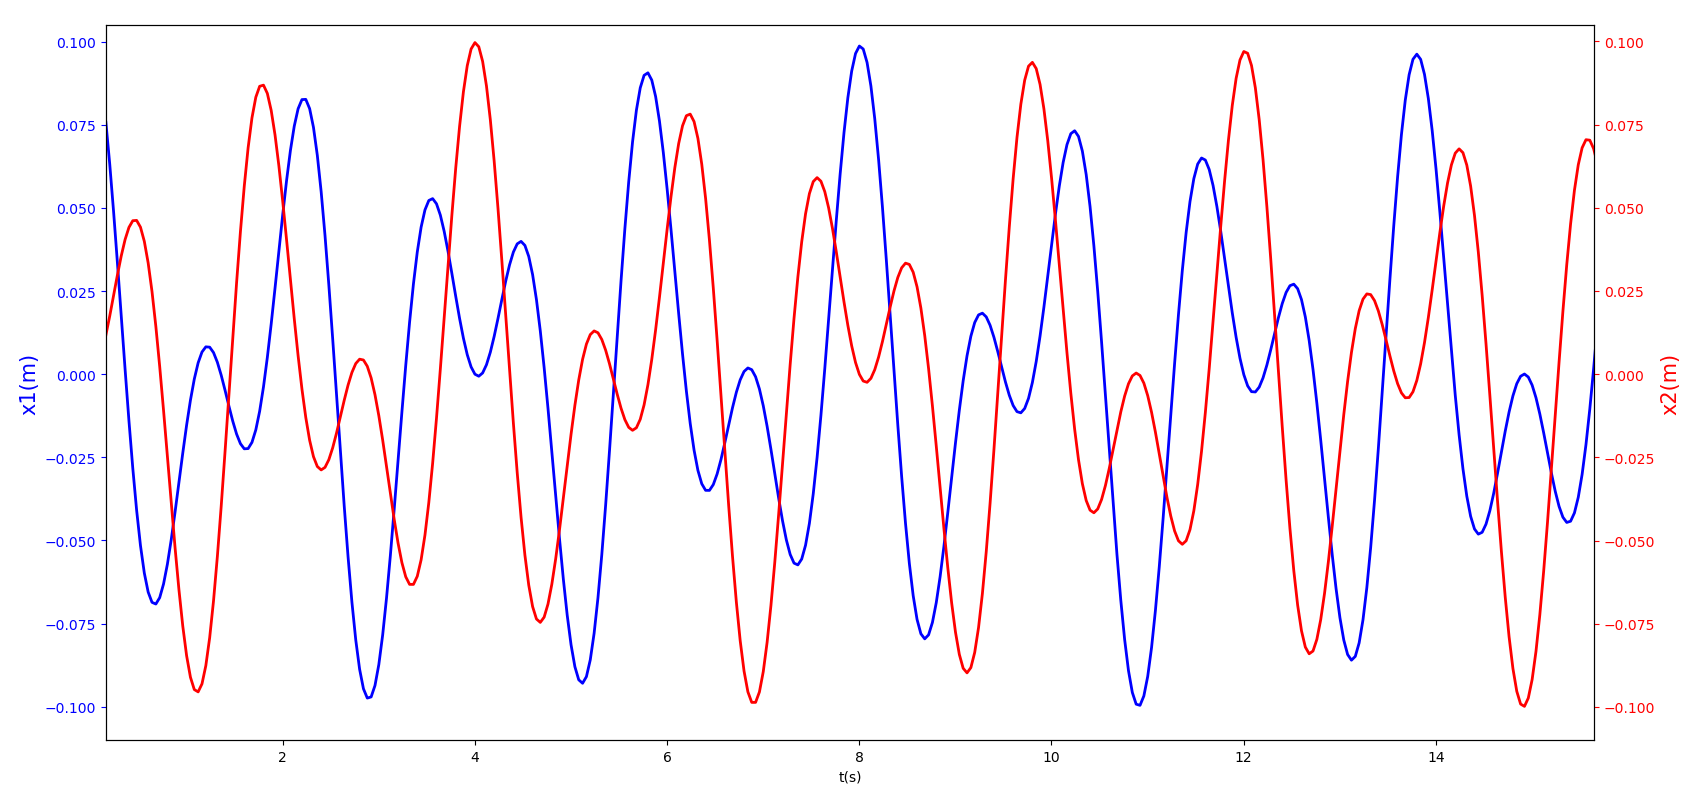
\includegraphics[width=0.8\textwidth]{posicion_k_iguales}
\caption{Posición masas respecto al tiempo $k'=k$}
\label{fig:1}
\end{figure}
Como podemos ver el movimiento parece un poco caótico pero si nos fijamos si que podemos ver un patrón. Observamos que ambas masas describen oscilaciones más amplias y otras más pequeñas que se deben a la influencia del muelle que une ambas masas. 
\begin{figure}[H]
    \centering
    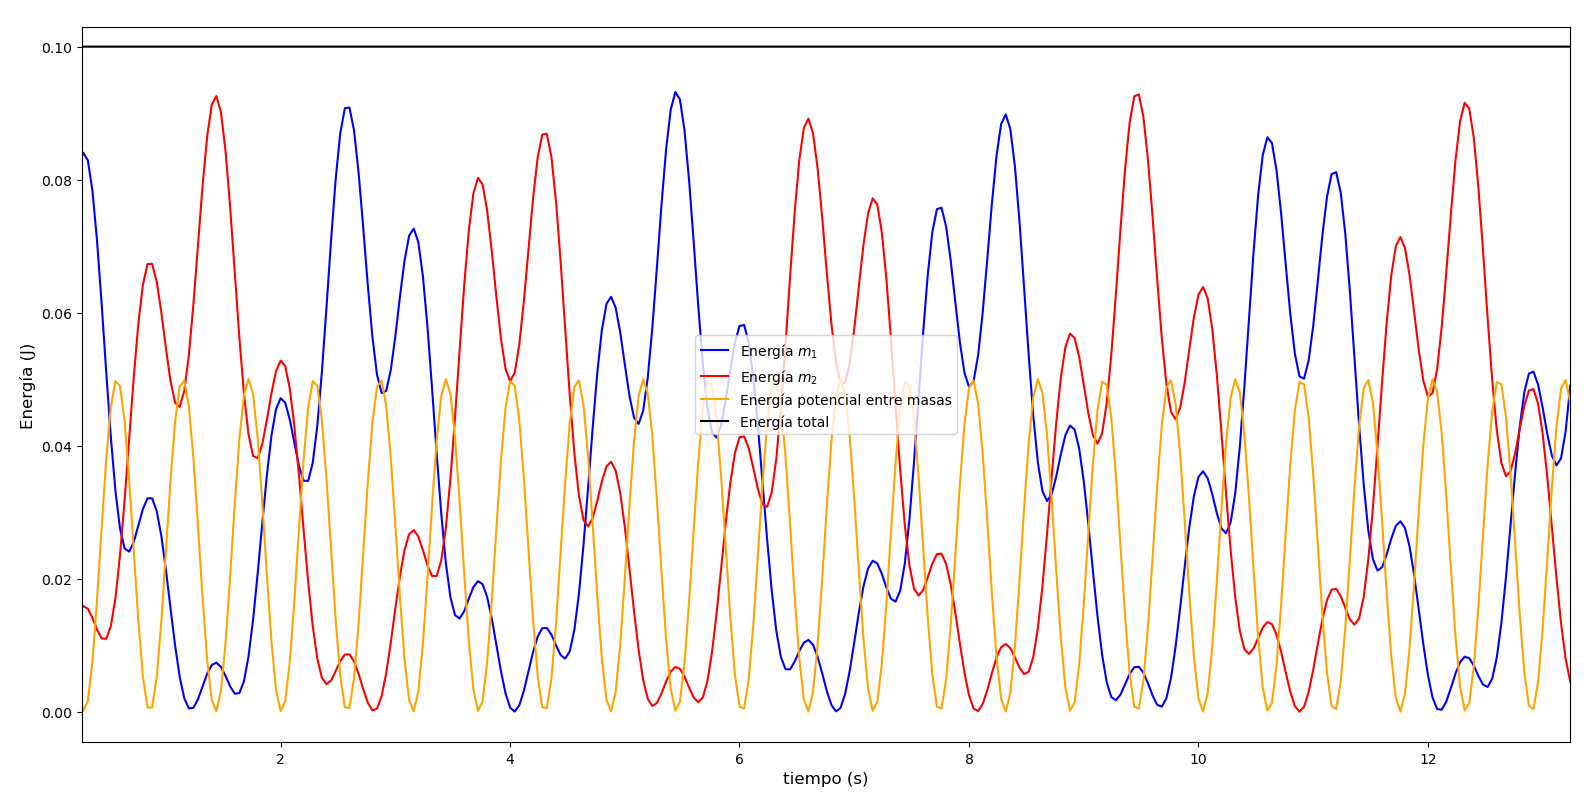
\includegraphics[width=0.8\textwidth]{energias_k_iguales}
\caption{Energías del sitema $k'=k$}
\label{fig:2}
\end{figure}
Si representamos las energías del sistema podemos ver que las energías totales de cada masa oscilan de una manera similar a su movimiento. También vemos que la energía potencial del muelle que une las masas si que es periódica. A pesar de todo esto podemos ver que la energía total del sistema es constante, cumpliendo así el principio de conservación de la energía.\newline\linebreak
Para obtener las frecuencias propias del sistema podemos hallar la transformada de Fourier:
\begin{figure}[H]
    \centering
    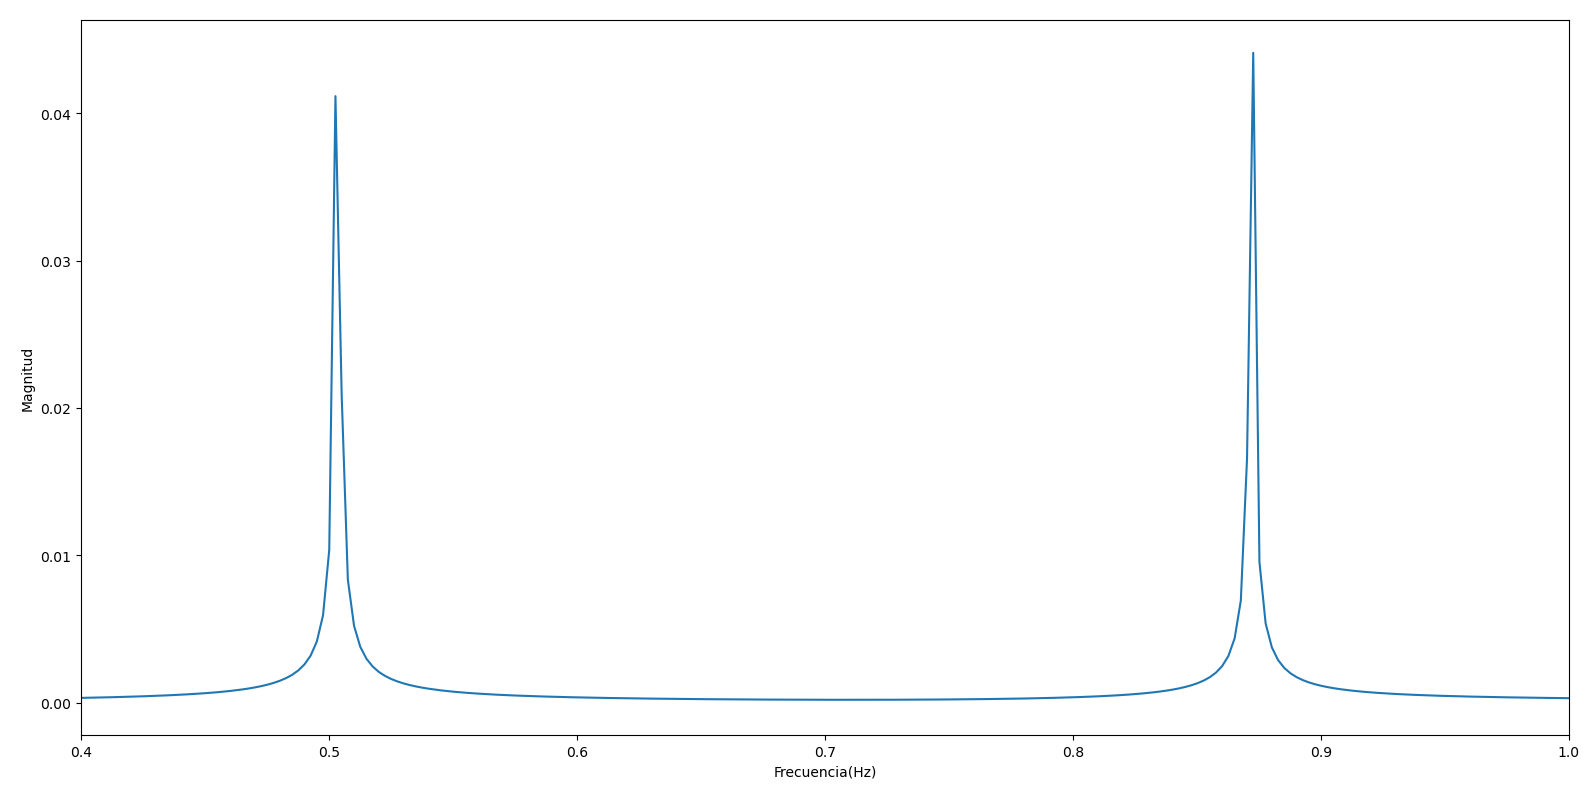
\includegraphics[width=0.8\textwidth]{fourier_k_iguales}
\caption{Transformada de Fourier del sitema $k'=k$}
\label{fig:f1}
\end{figure}
En la figura podemos ver dos picos que representan las dos frecuencias características del sistema. Vemos que rondan los $0.51\hspace{0.1cm} Hz$ y los $0.87\hspace{0.1cm} Hz$, si de aquí calculamos las frecuencias angulares mediante la fórmula $\omega = 2\pi f$ obtenemos que $\omega_1 = 3.14 \hspace{0.1cm}rad/s$ y $\omega_2 = 5.34\hspace{0.1cm}rad/s$. Además, si las calculamos teóricamente con las ecuaciones que hemos obtenido (\ref{ec.:5}) tenemos que:
$$\omega_1 = 3.16\hspace{0.1cm}rad/s \hspace{2cm}y\hspace{2cm}  \omega_2 = 5.47\hspace{0.1cm}rad/s$$
lo que indica que la Transformada de Fourier es una manera rápida y adecuada de calcular gráficamente las frecuencias características del sistema en cada caso.\newline\linebreak
\noindent$\tcboxmath[colback=blue!10!white,colframe=blue!25!white]{\bullet\hspace{0.2cm} k'>k\hspace{14cm}}\label{ec.:4}$\newline\linebreak
Si consideramos ahora un valor para $k'$ mayor que $k$ ($k'=30\hspace{0.1cm}N/m$), vemos que las masas están ligadas más fuertemente, es decir, como podemos ver en la Figura \ref{fig:3} cuando la masa 1 está en un mínimo la masa 2 está en un máximo y vicerversa pero vemos que la distancia entre ambas masas es prácticamente la misma en todo momento.\newline\linebreak

\begin{figure}[H]
    \centering
    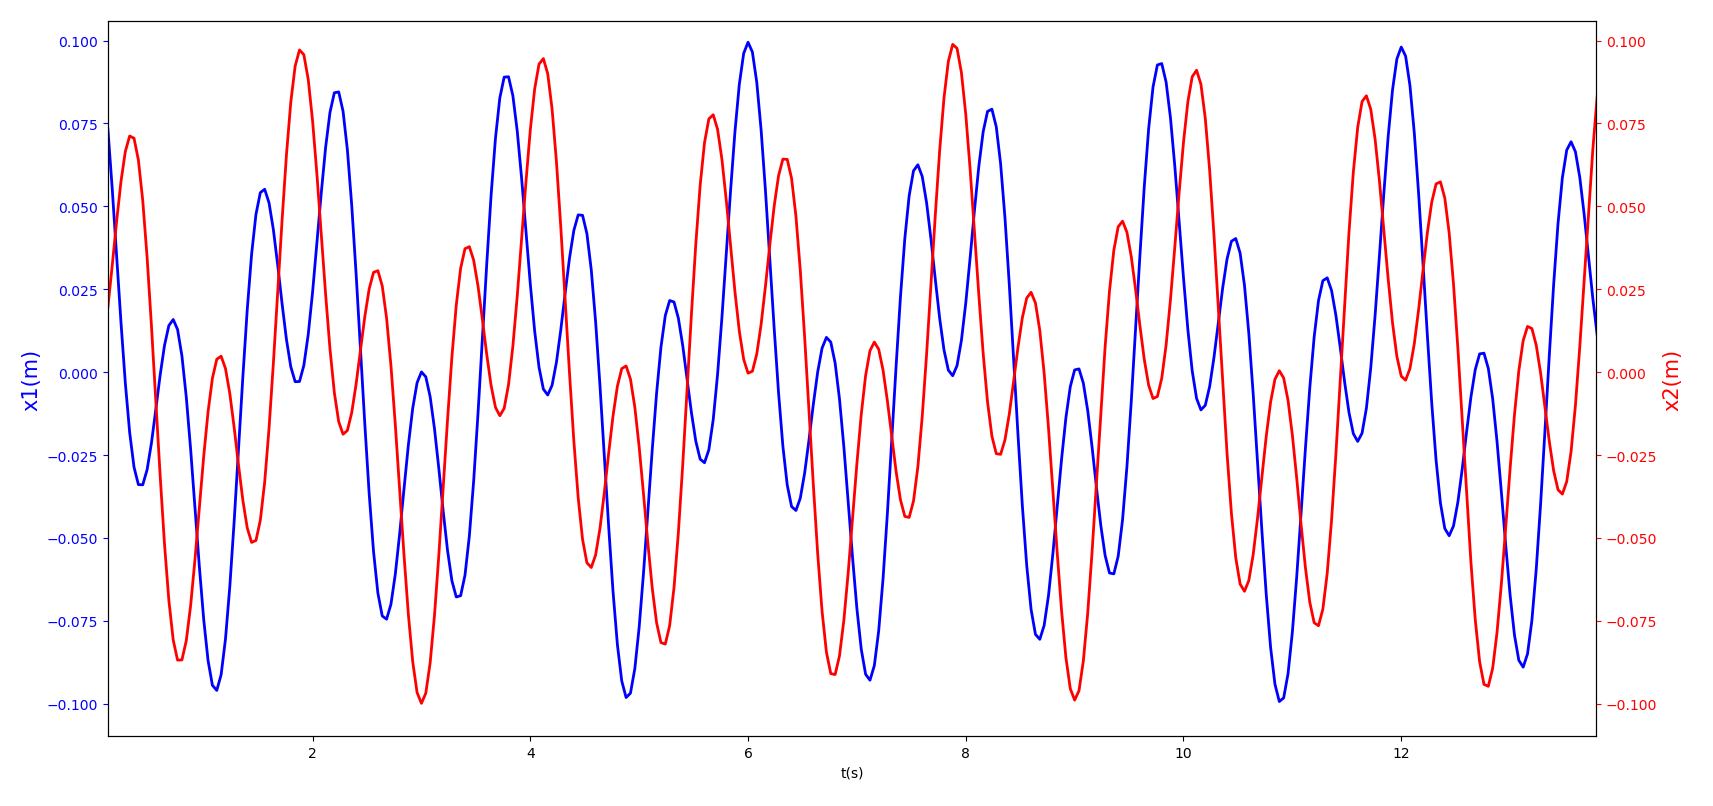
\includegraphics[width=0.8\textwidth]{posicion_k_mayor}
\caption{Posición masas respecto al tiempo $k'>k$}
\label{fig:3}
\end{figure}
Al representar las energías del sistema (Figura \ref{fig:4}) vemos que la energía total del sistema es constante pero su magnitud es mayor que cuando coincidían los valores de las constantes elásticas de los tres muelles.\newline\linebreak
Si comparamos con el caso anterior podemos ver que la amplitud máxima de las oscilaciones es la misma en ambos casos pero en este segundo caso, al estar las masas "más ligadas", la frecuencia de oscilación va a ser mayor, como podemos ver en la figura \ref{fig:f2} de donde obtenemos unas frecuencias angulares de oscilación de $3.16 \hspace{0.1cm}rad/s$ y $6.32 \hspace{0.1cm}rad/s$. Vemos que una de las frecuencias siempre va a ser igual ya que se calcula mediante la $k$ que en nuestro caso va a mantenese fija.\newline\linebreak
A consecuencia de que la frecuencia de oscilación del sistema sea más alta se produce un aumento de energía  del sistema. Como podemos comprobar en la figura \ref{fig:5} en este caso la energía total del sistema va a valer $0.2\hspace{0.1cm}J$ mientras que en el anterior sistema valía $0.1\hspace{0.1cm}J$
\begin{figure}[H]
    \centering
    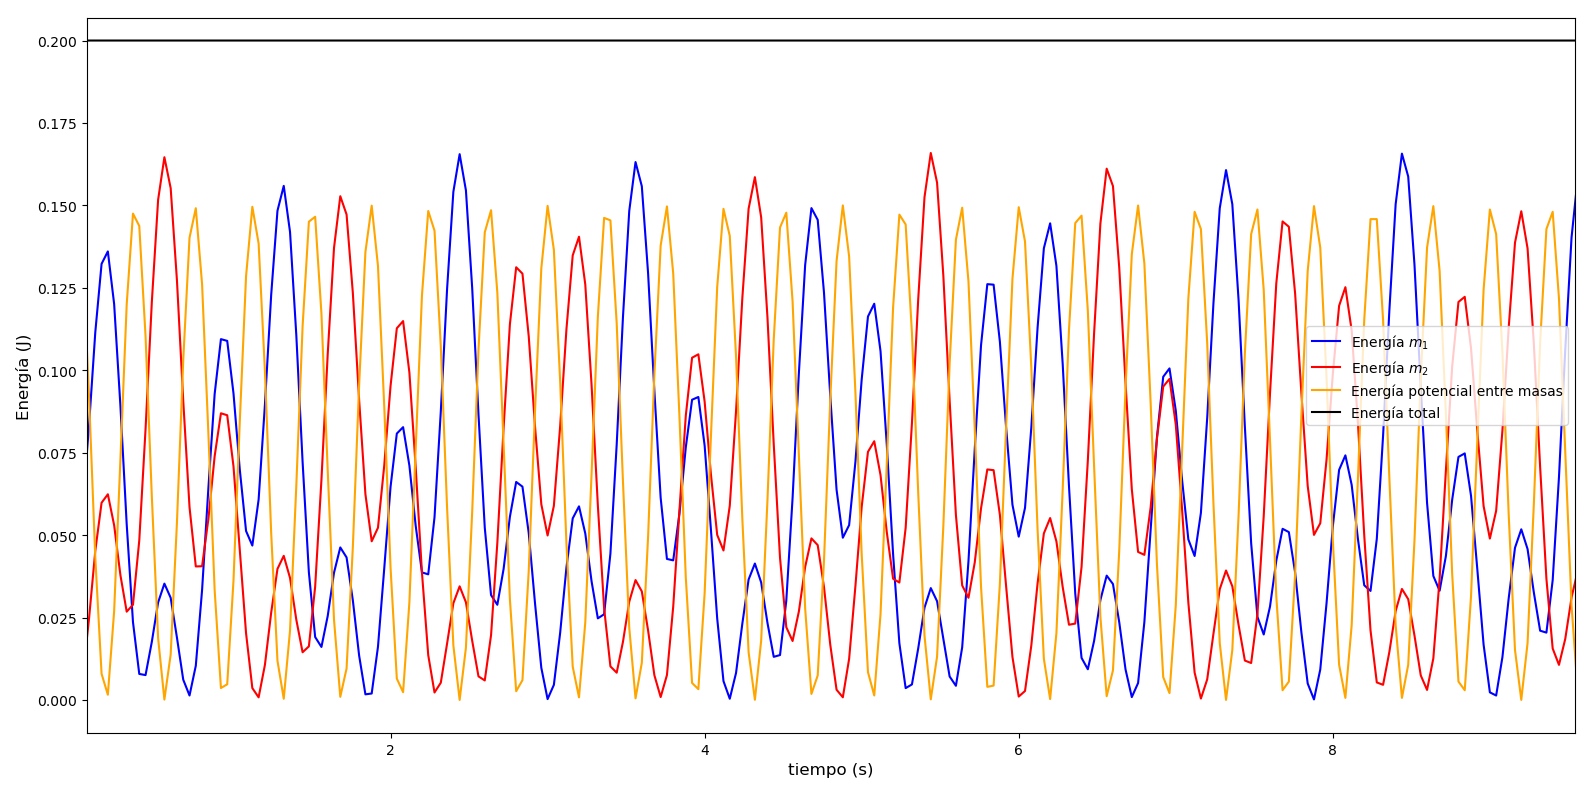
\includegraphics[width=0.8\textwidth]{energias_k_mayor}
\caption{Energías del sitema $k'>k$}
\label{fig:4}
\end{figure}
\begin{figure}[H]
    \centering
    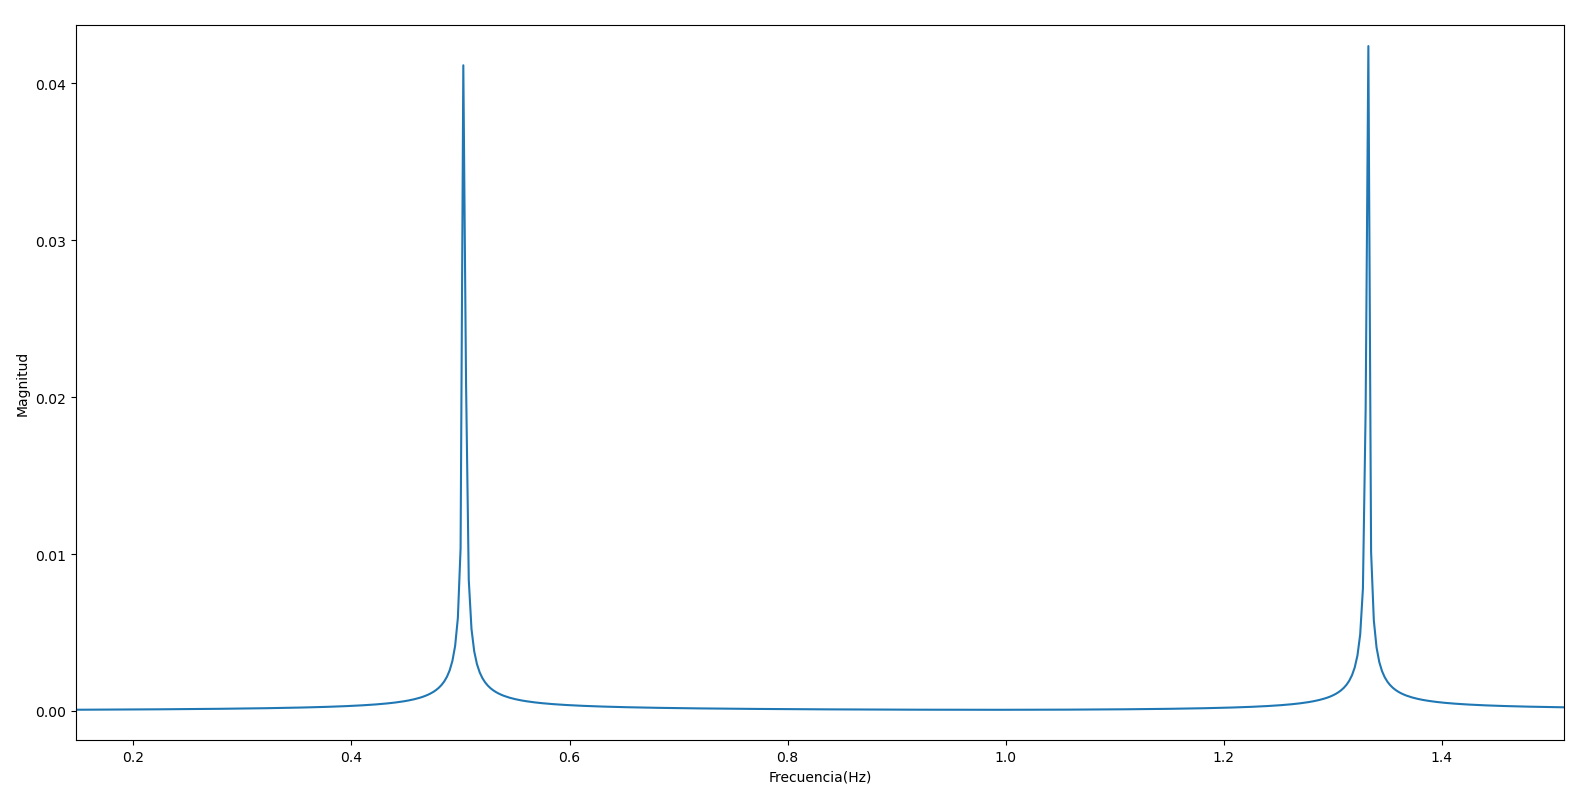
\includegraphics[width=0.8\textwidth]{fourier_k_mayor}
\caption{Transformada de Fourier del sitema $k'>k$}
\label{fig:f1}
\end{figure}
\vspace{2cm}
\noindent$\tcboxmath[colback=blue!10!white,colframe=blue!25!white]{\bullet\hspace{0.2cm} k'\ggg k\hspace{14cm}}\label{ec.:4}$\newline\linebreak
Tomando una $k' = 200\hspace{0.1cm}N/m$ mucho mayor que $k$ podemos ver que el acomplamiento entre las masas va a ser muy fuerte, viendo en este caso que se conserva la distancia entre ambas masas en todo momento, como si estuvieran unidas por una varilla inextensible. Además, por esto la frecuencia de oscilación va a ser mucho más alta que en los casos anteriores, situándose en $14.5\hspace{0.1cm}rad/s$ y, como ya hemos dicho, aumenta la energía del sistema que permanece constante en $1.1\hspace{0.1cm}J$.

\begin{figure}[H]
\centering
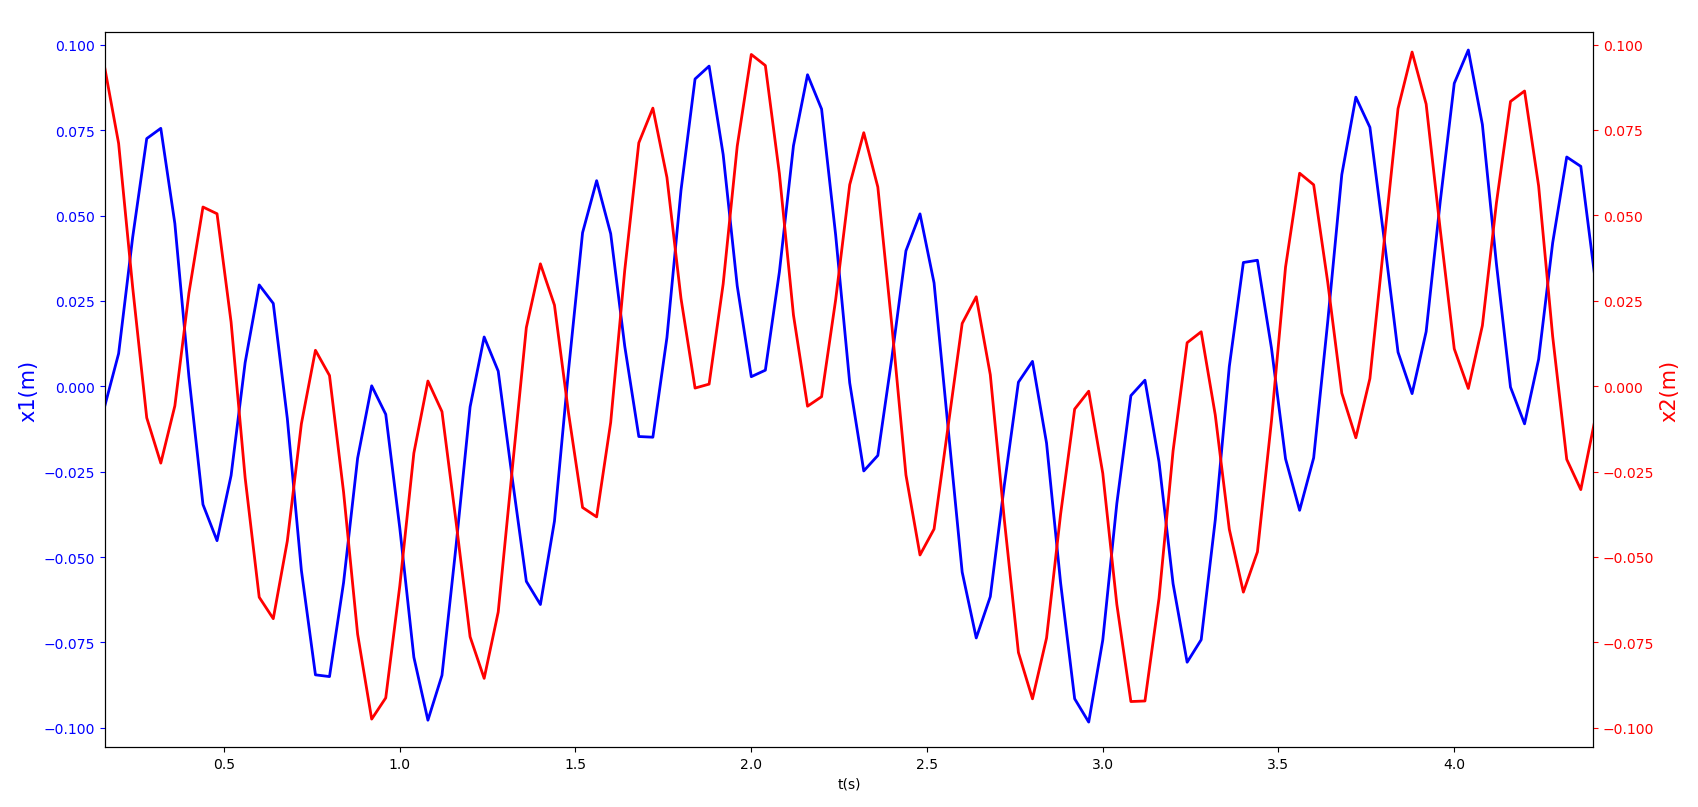
\includegraphics[width=0.8\textwidth]{posicion_k_mas_mayor}
\caption{Posición masas respecto al tiempo $k'\ggg k$}
\label{fig:5}
\end{figure}
\begin{figure}[H]
\centering
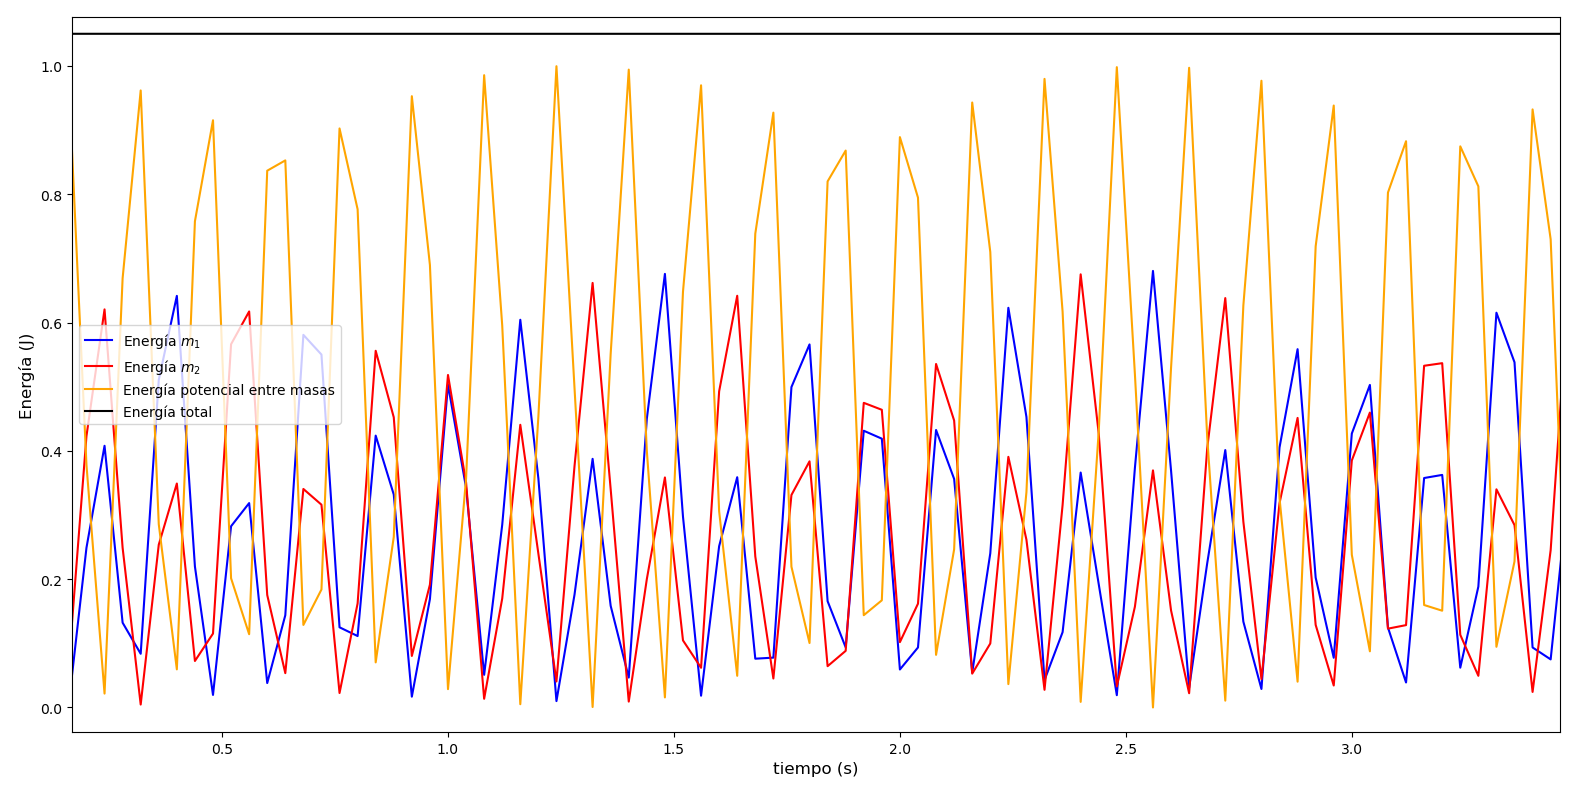
\includegraphics[width=0.8\textwidth]{energias_k_mas_mayor}
\caption{Energías del sitema $k'\ggg k$}
\label{fig:6}
\end{figure}
\begin{figure}[H]
    \centering
    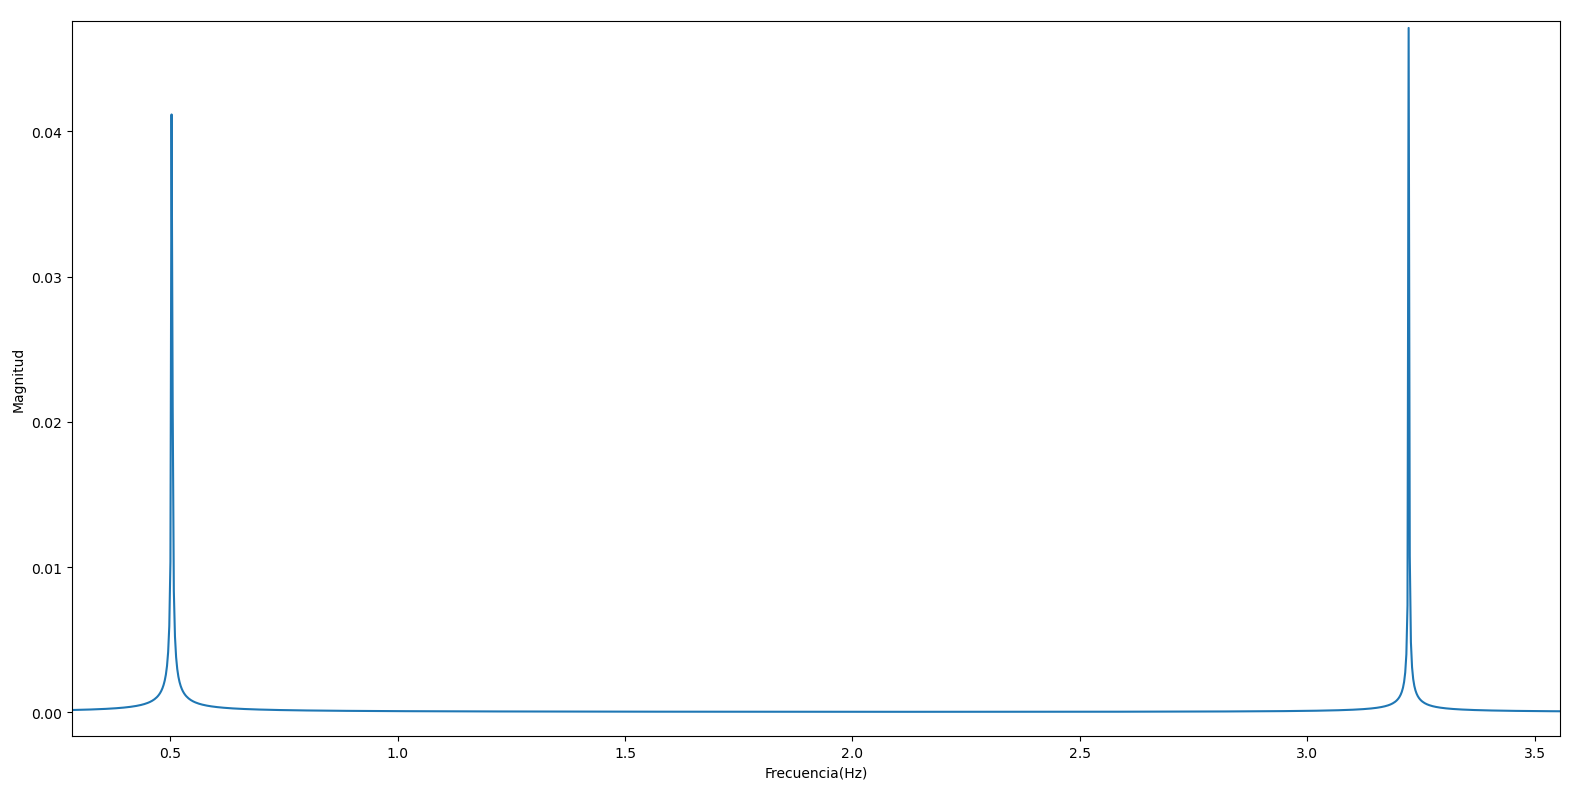
\includegraphics[width=0.8\textwidth]{fourier_k_mas_mayor}
\caption{Transformada de Fourier del sitema $k'\ggg k$}
\label{fig:f3}
\end{figure}


$\tcboxmath[colback=blue!10!white,colframe=blue!25!white]{\bullet\hspace{0.2cm} k'<k\hspace{14cm}}\label{ec.:4}$\newline\linebreak
Ahora vamos a ver que ocurre cuando la constante elástica del muelle que une ambas masas es más pequeña que la de los muelles que unen estas a las paredes.
\begin{figure}[H]
    \centering
    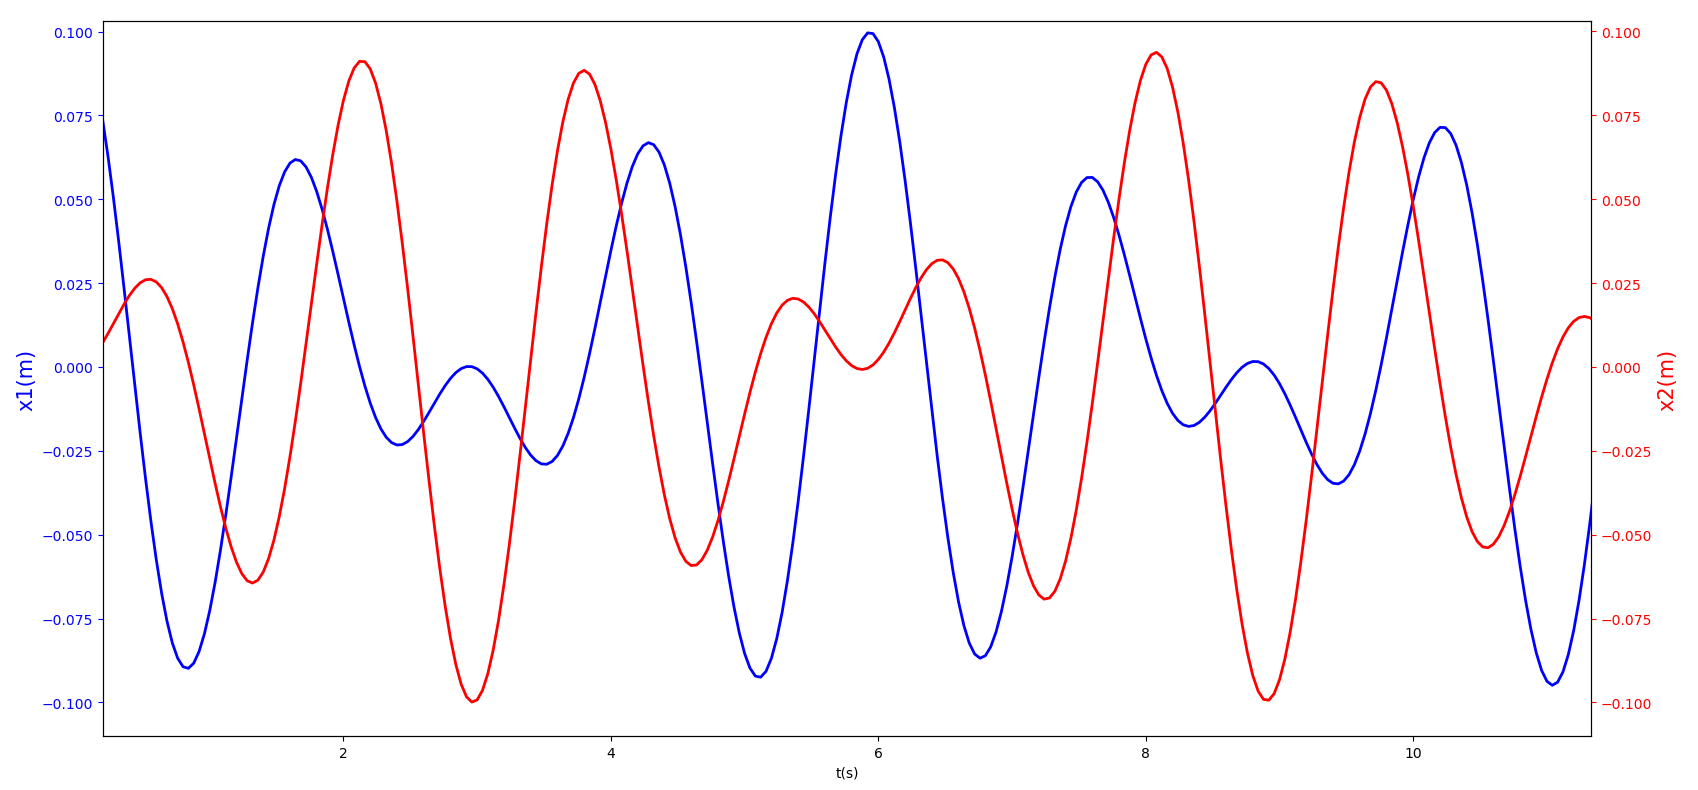
\includegraphics[width=0.8\textwidth]{posicion_k_menor}
\caption{Posición masas respecto al tiempo $k'<k$}
\label{fig:7}
\end{figure}
Como vemos ahora si que podemos ver oscilaciones completas de las masas claramente y vemos que la influencia del muelle central es mucho menor, por lo que las masas se mueven más independientemente, no están tan acopladas como en los casos anteriores. Y en este caso obtenemos unas frecuencias propias de $\omega_1 = \sqrt{10}\hspace{0.1cm}rad/s$ y $\omega_1 = \sqrt{14}\hspace{0.1cm}rad/s$
\begin{figure}[H]
    \centering
    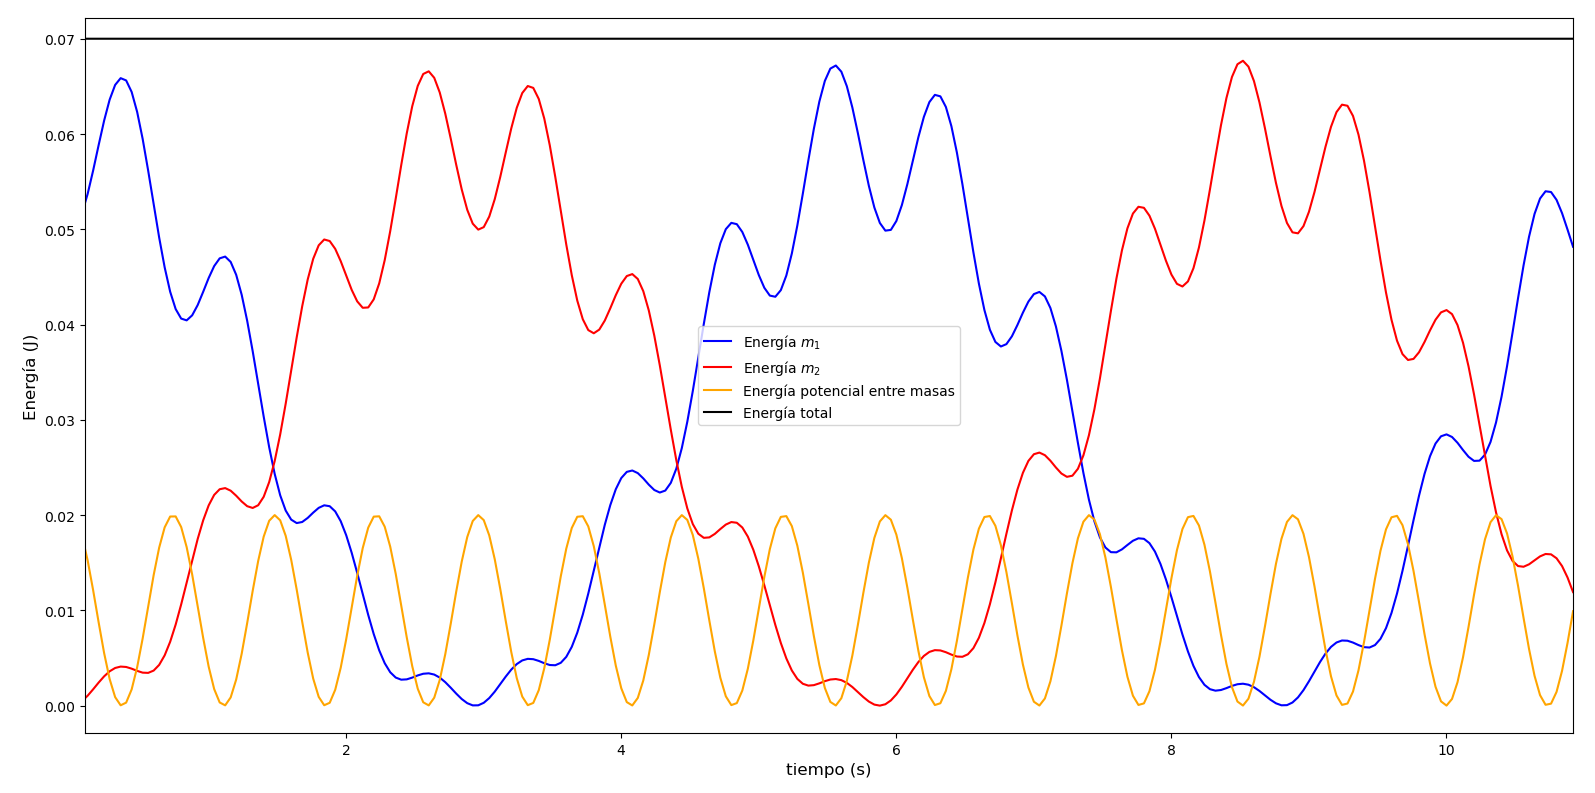
\includegraphics[width=0.8\textwidth]{energias_k_menor}
\caption{Energías del sitema $k'<k$}
\label{fig:8}
\end{figure}
Si representamos las energías del sistema vemos que, como en todos los casos, la energía mecánica del sistema se conserva y en este caso, es más baja que en los casos anteriores.\newline\linebreak

$\tcboxmath[colback=blue!10!white,colframe=blue!25!white]{\bullet\hspace{0.2cm} k'\lll k\hspace{14cm}}\label{ec.:4}$\newline\linebreak
Por último, vamos a considerar el caso de acoplamiento débil, tomando una $k'=0.5\hspace{0.1cm}N/m$.
\begin{figure}[H]
    \centering
    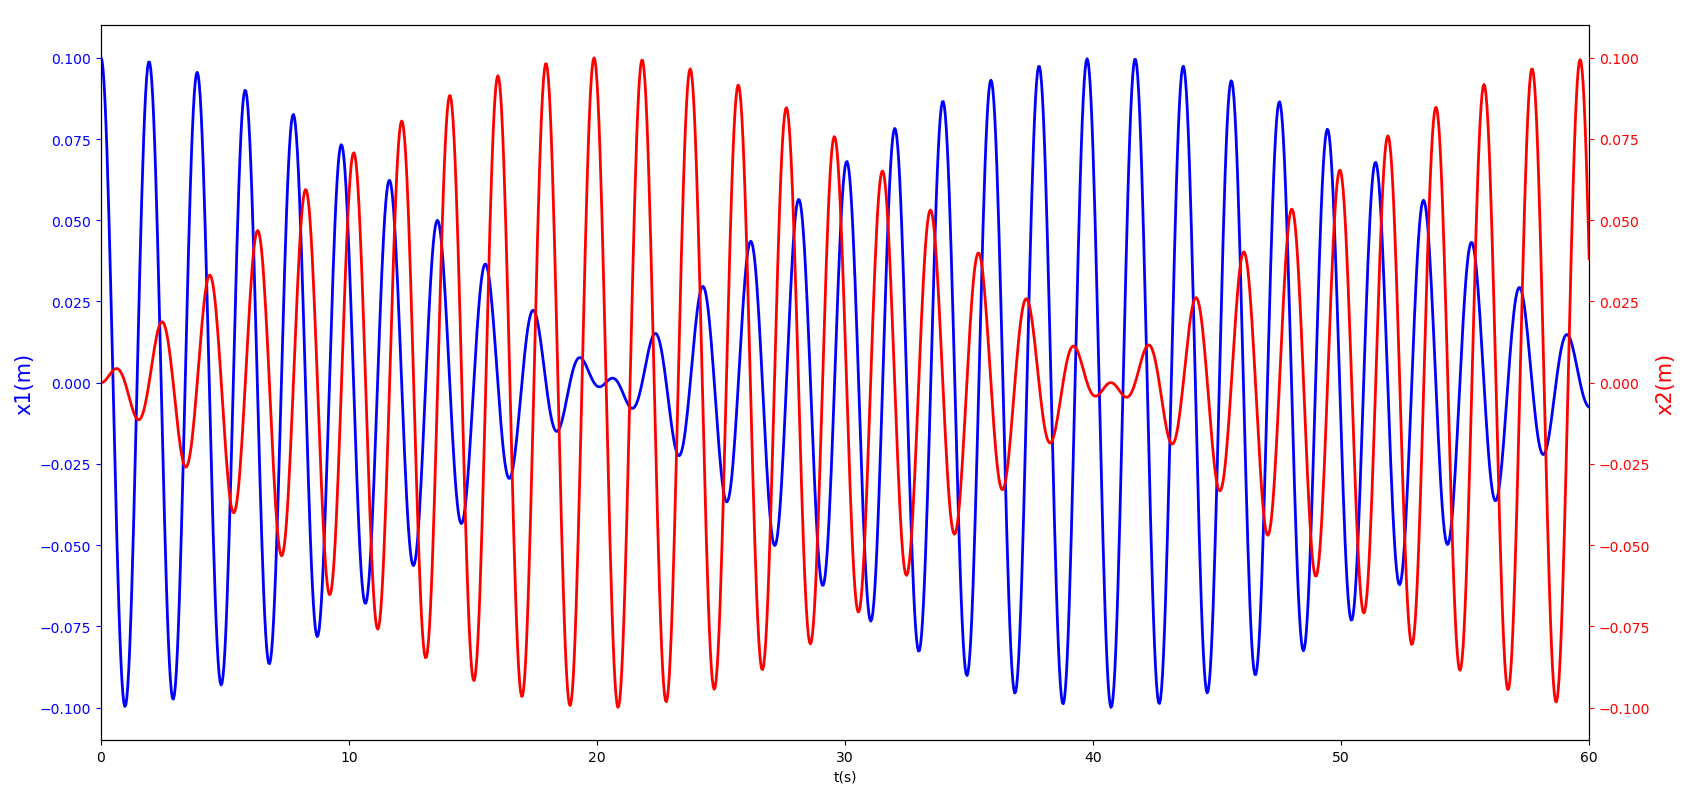
\includegraphics[width=0.8\textwidth]{posicion_k_mas_menor}
\caption{Posición masas respecto al tiempo $k'\lll k$}
\label{fig:9}
\end{figure}
En la Figura \ref{fig:9} podemos ver representada la posición de las masas frente al tiempo. En este caso vemos que el muelle central permite mucha más libertad a las masas, dándose un fenómeno llamado pulsos de batido que viene dado por las ecuaciones (\ref{ec.:9}) y (\ref{ec.:10}). En la figura \ref{fig:12} podemos ver que el periodo de batido del sistema, es decir, el tiempo que tarda cada una de las masas en oscilar completamente entre dos posiciones extremas, va a ser aproximadamente de unos 40 segundos.\newline\linebreak
En lo que se refiere a las energías del sistema vemos que como es esperado la energía total del sistema se conserva además de ser más baja que en los casos anteriores. En esta figura también se observa de manera muy clara la transferencia de energía entre las dos masas.
\begin{figure}[H]
    \centering
    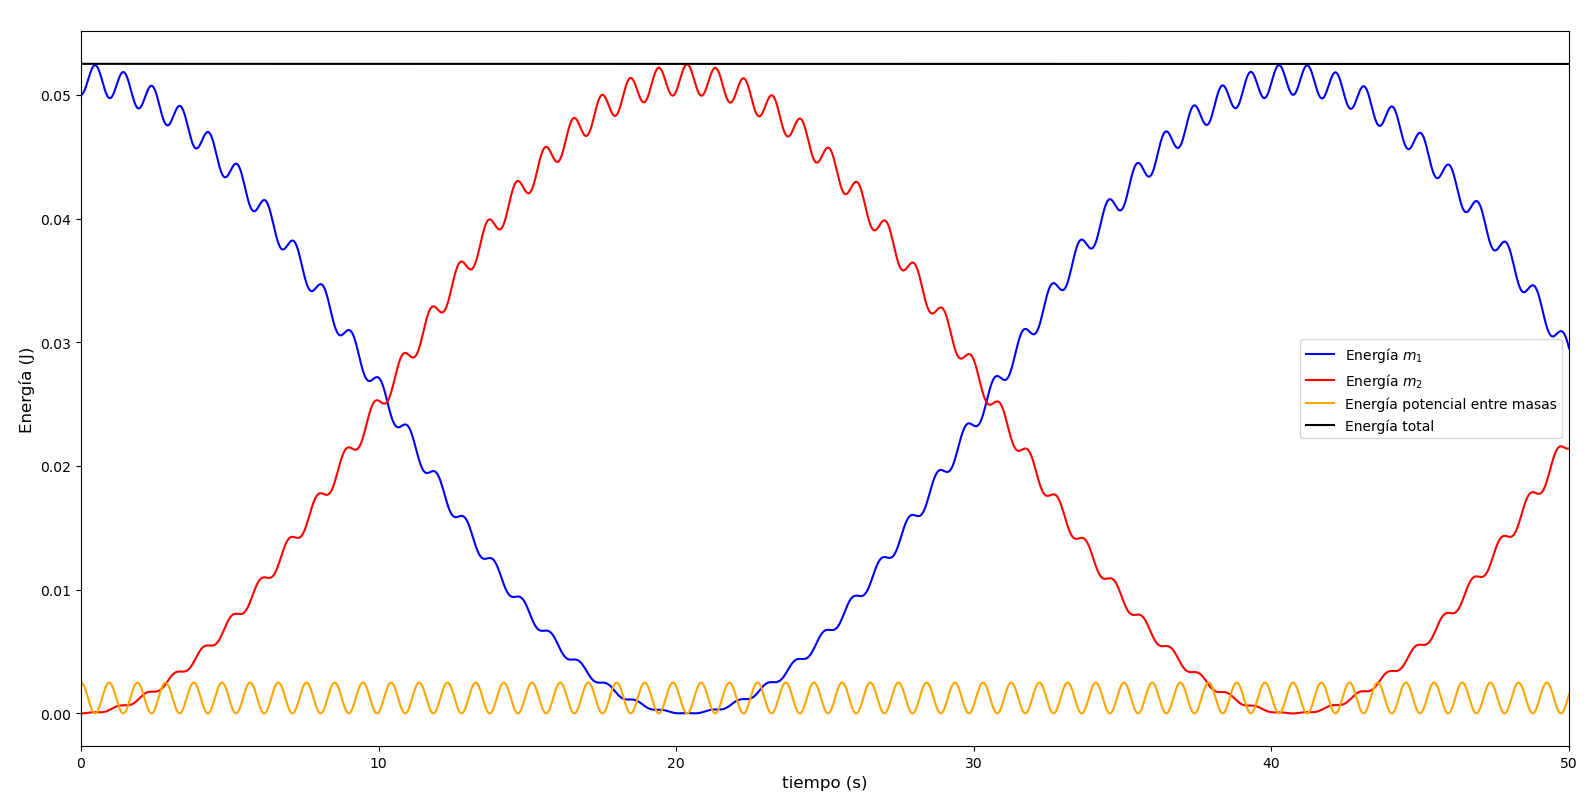
\includegraphics[width=0.8\textwidth]{energias_k_mas_menor}
\caption{Energías del sitema $k'\lll k$}
\label{fig:10}
\end{figure}
\begin{figure}[H]
    \centering
    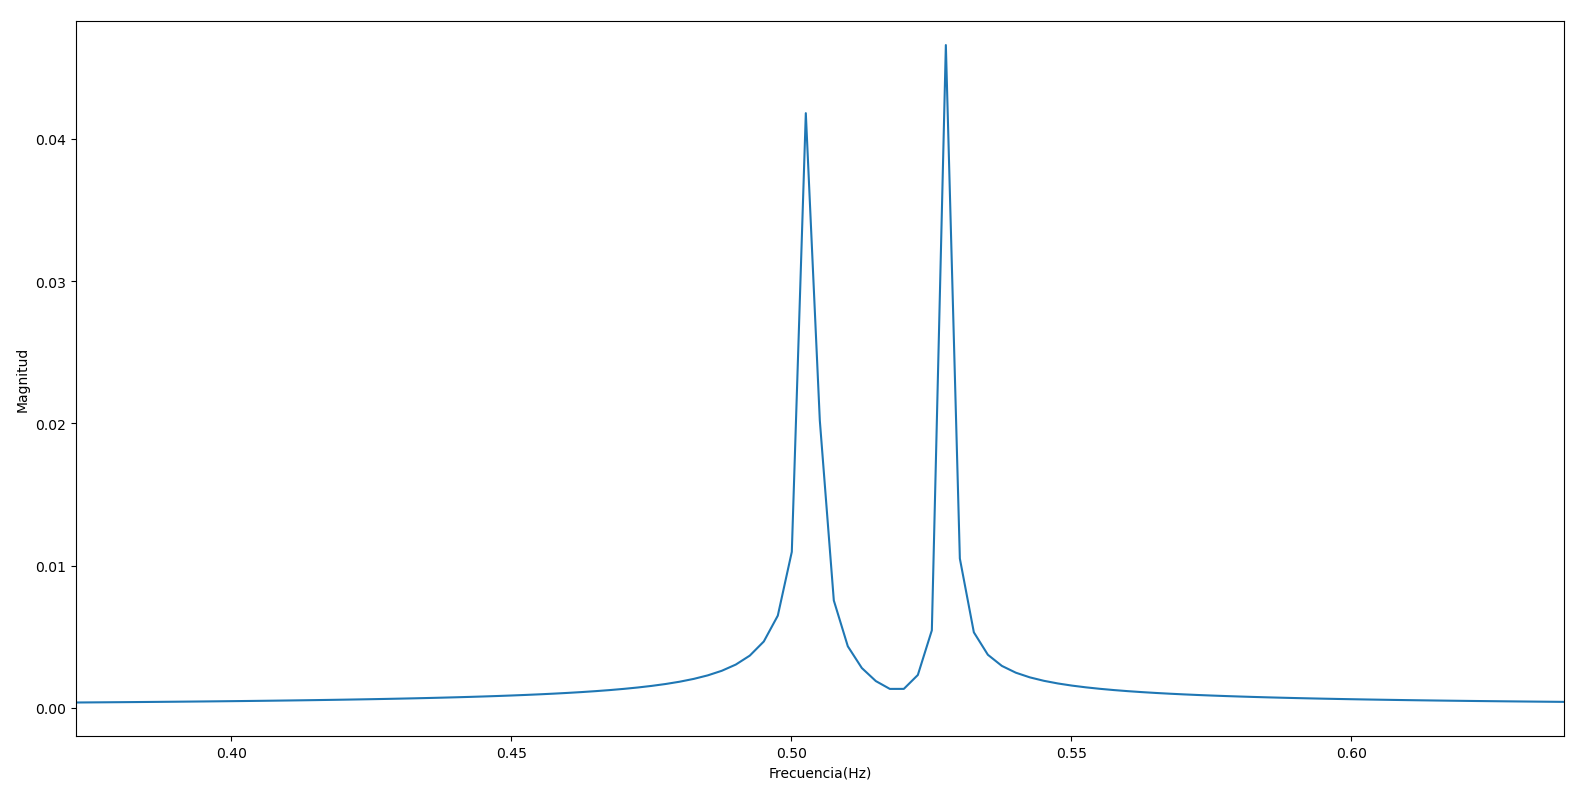
\includegraphics[width=0.8\textwidth]{fourier_k_mas_menor}
\caption{Transformada de Fourier del sitema $k'\lll k$}
\label{fig:f}
\end{figure}
Si observamos la Transformada de Fourier del sistema podemos ver que, como habíamos predicho, las frecuencias propias del sistema son muy parecidas debido a que $k'$ va a sr mucho más pequeña que $k$.
\section{Modos normales}
Ahora vamos a ver cómo se comporta el sistema cuando excitamos los modos normales de oscilación.
\subsection{Modo simétrico de vibración}
Para el modo simétrico vamos a considerar como condiciones iniciales $x_1(0)=x_2(0)=0\hspace{0.1cm}m$ y $\dot{x_1}(0)=\dot{x_2}(0)=1\hspace{0.1cm}m/s$
\begin{figure}[H]
\centering
\begin{subfigure}[b]{0.45\linewidth}
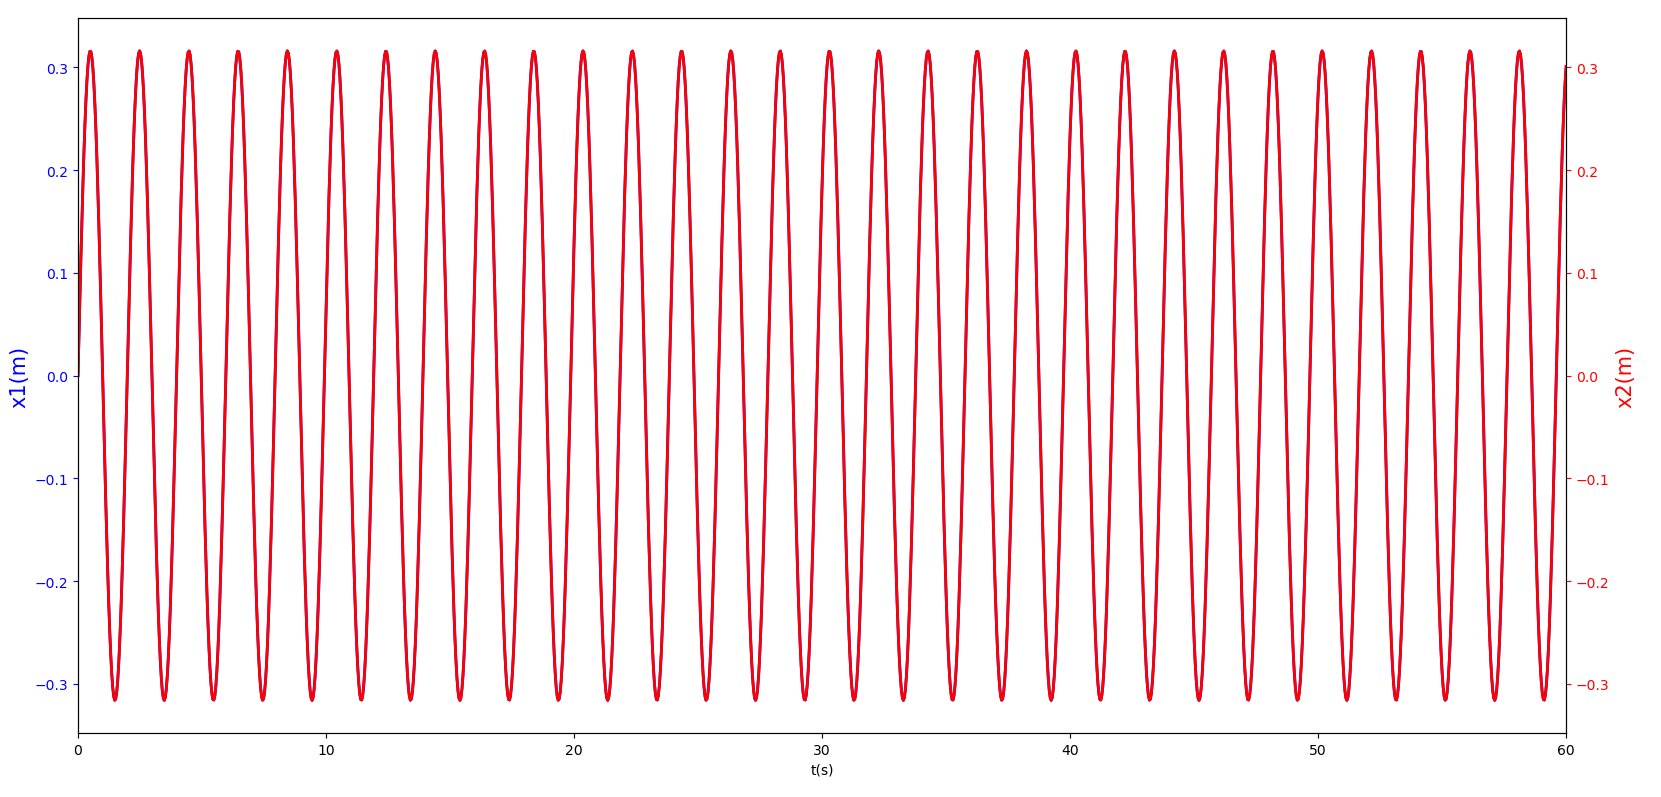
\includegraphics[width=\linewidth]{simetrico_debil}
\caption{$k' = 0.5$}
\label{fig:3a}
\end{subfigure}
\begin{subfigure}[b]{0.45\linewidth}
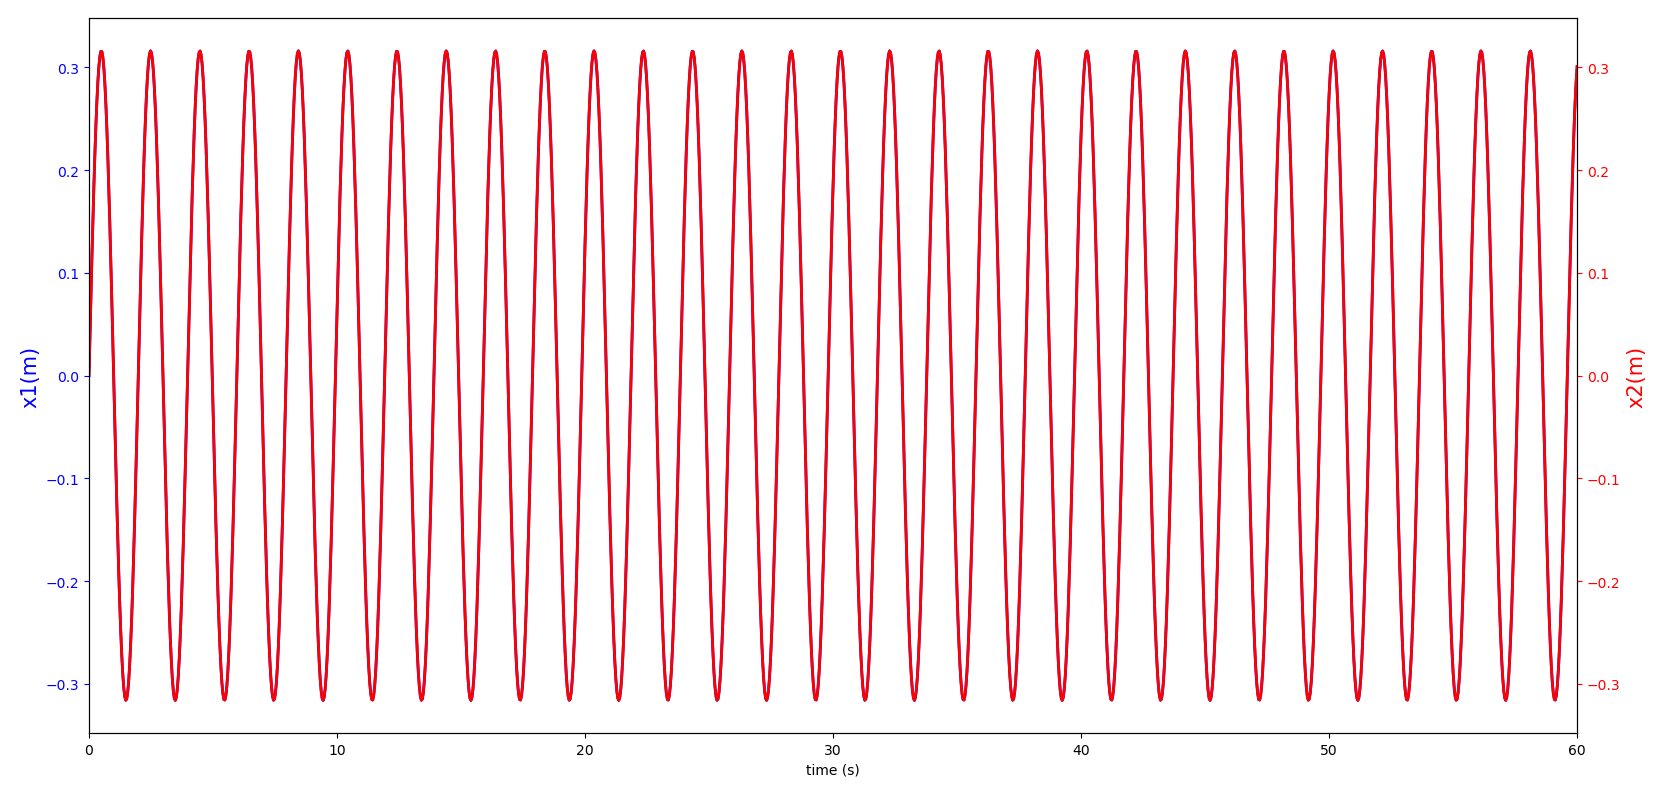
\includegraphics[width=\linewidth]{simetrico_k_iguales}
\caption{$k' = 10$}
\label{fig:3b}
\end{subfigure}
\caption{Modo normal simétrico}
\label{fig:15}
\end{figure}
En la Figura \ref{fig:15} podemos ver el movimiento de las masas en función del tiempo para $k = 10$ y $k'=0.5$ y $k'=10$ respectivamente. Al ver esto podemos deducir que el movimento del sistema va a ser igual independientemente de los valores que le asignemos a la constante elástica $k'$. Esto se debe a que ambas masas van a oscilar en fase y la frecuencia de oscilación del sistema va a venir dada por $\omega = \sqrt{k/m}$, que depende solo de la masa y la k del muelle que une una de las masas a la pared. De ahí que si observamos la Figura \ref{fig:17} veamos un único pico, ya que solo existe un modo de oscilación del sitema.
\begin{figure}[H]
\centering
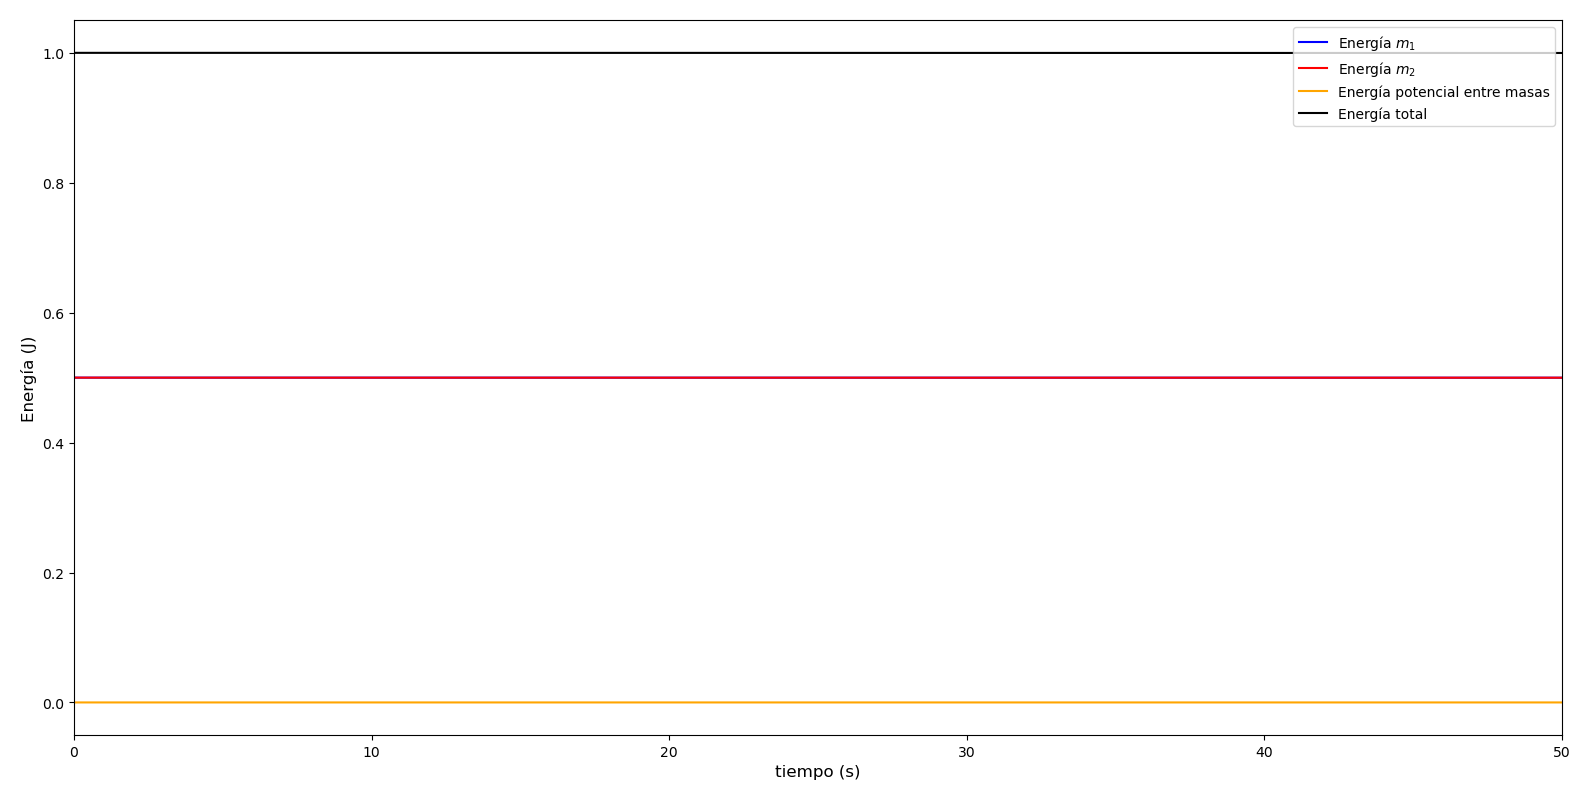
\includegraphics[width=0.7\textwidth]{simetrico_energias_debil}
\caption{Energías modo normal simétrico}
\label{fig:3}
\end{figure}

\begin{figure}[H]
\centering
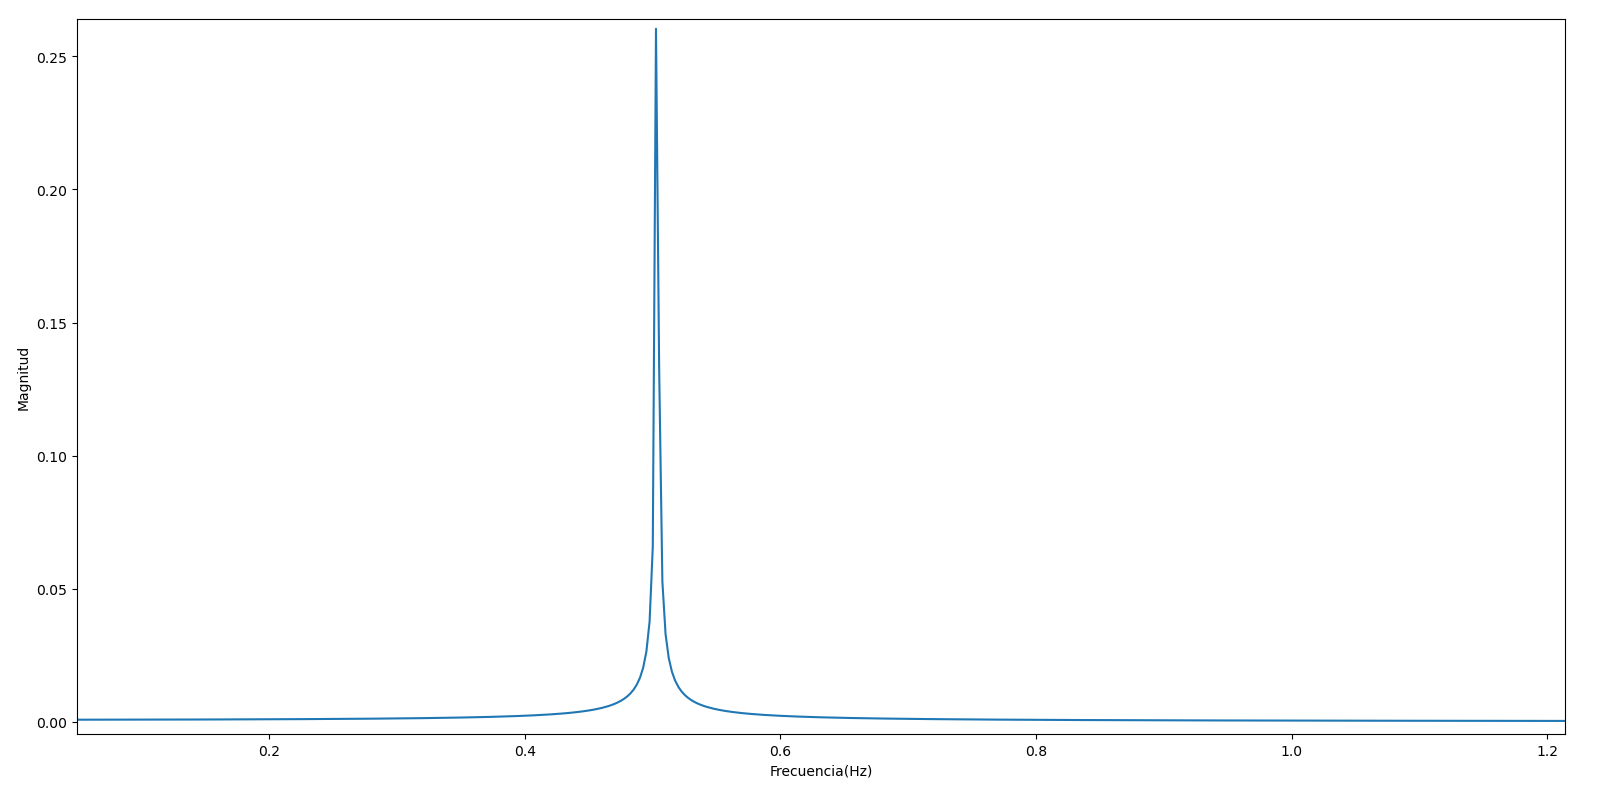
\includegraphics[width=0.7\textwidth]{simetrico_fourier_debil}
\caption{Transformada de Fourier modo simétrico}
\label{fig:17}
\end{figure}
También es interesante observar que en este caso, al oscilar las dos masas en fase las energías de cada componente del sistema se van a mantener constantes al igual que la energía potencial del muelle que une ambas masas va a ser 0.
\subsection{Modo antisimétrico de vibración}
Para excitar el modo normal antisimétrico hemos considerado $x_1(0)=-x_2(0)=0\hspace{0.1cm}m$ y $\dot{x_1}(0)=-\dot{x_2}(0)=1\hspace{0.1cm}m/s$ 
\begin{figure}[H]
\centering
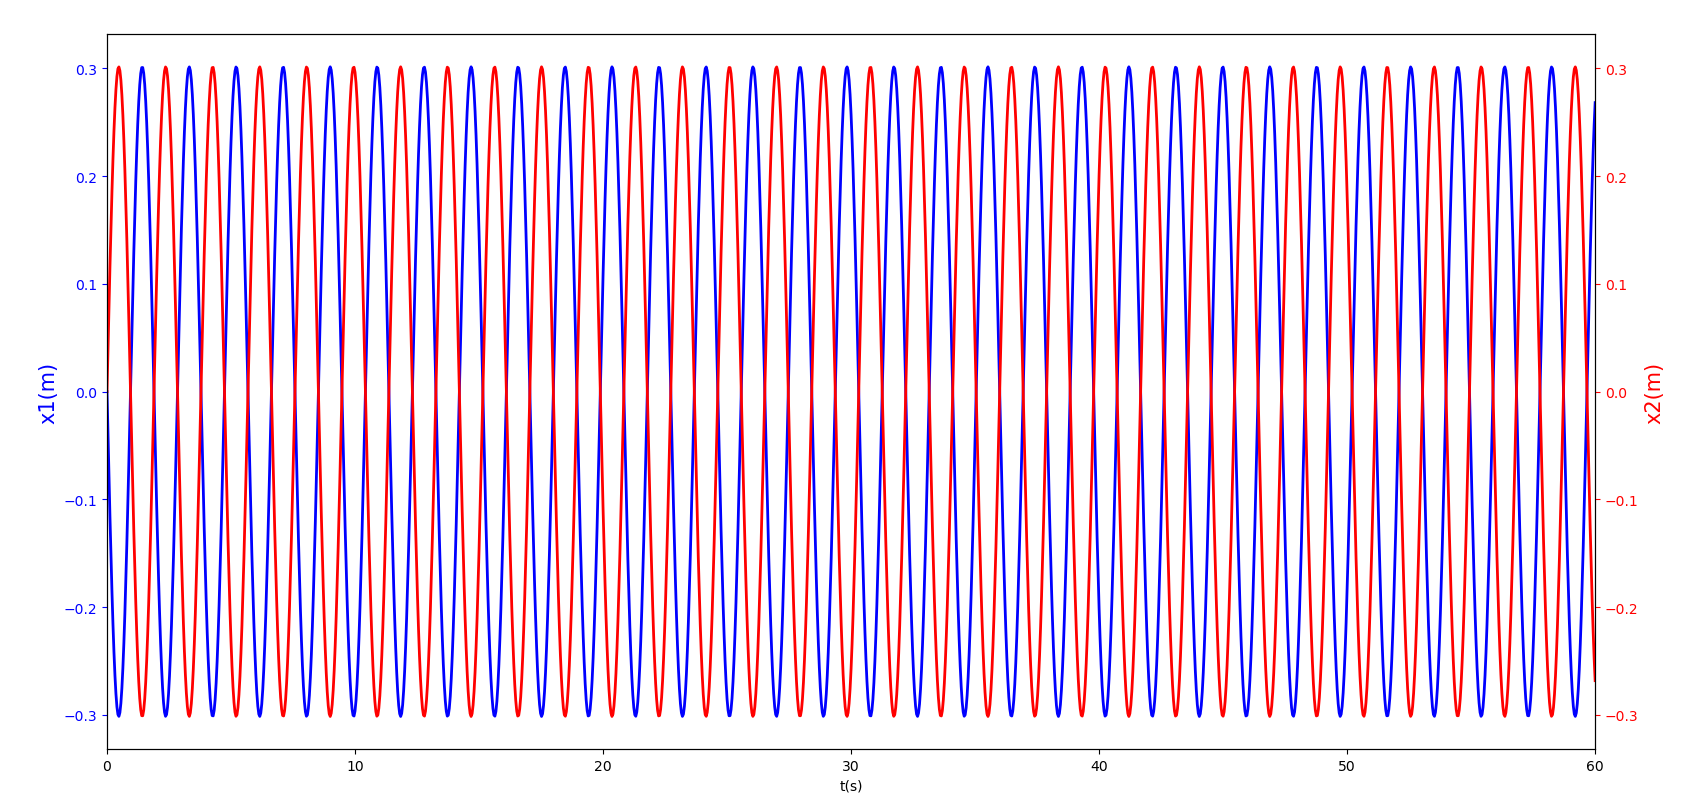
\includegraphics[width=0.8\textwidth]{antisimetrico}
\caption{ Modo normal antisimétrico}
\label{fig:3}
\end{figure}
Como podemos ver en la figura en este modo las masas van a vibrar a la misma frecuencia pero en este caso en oposición de fase. Al ocurrir esto vemos que sí que va a haber transferencias de energía entre las masas, que ambas tienen la misma energía, y la energía potencial del muelle manteniendo así la energía total del sistema constante.
\begin{figure}[H]
\centering
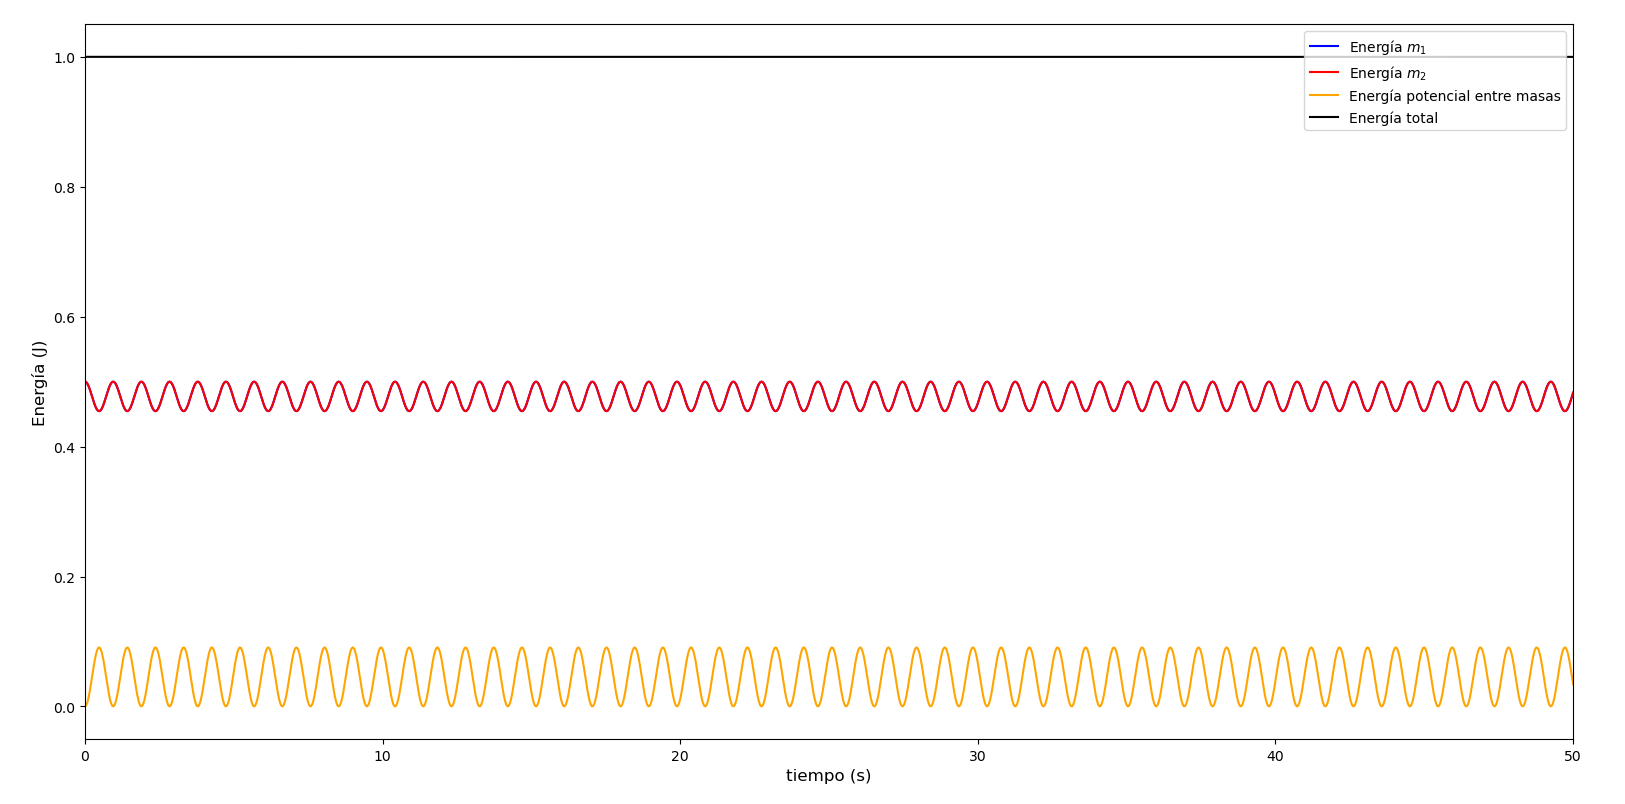
\includegraphics[width=0.8\textwidth]{antisimetrico_energias}
\caption{Energías modo normal antisimétrico}
\label{fig:3}
\end{figure}
\begin{figure}[H]
\centering
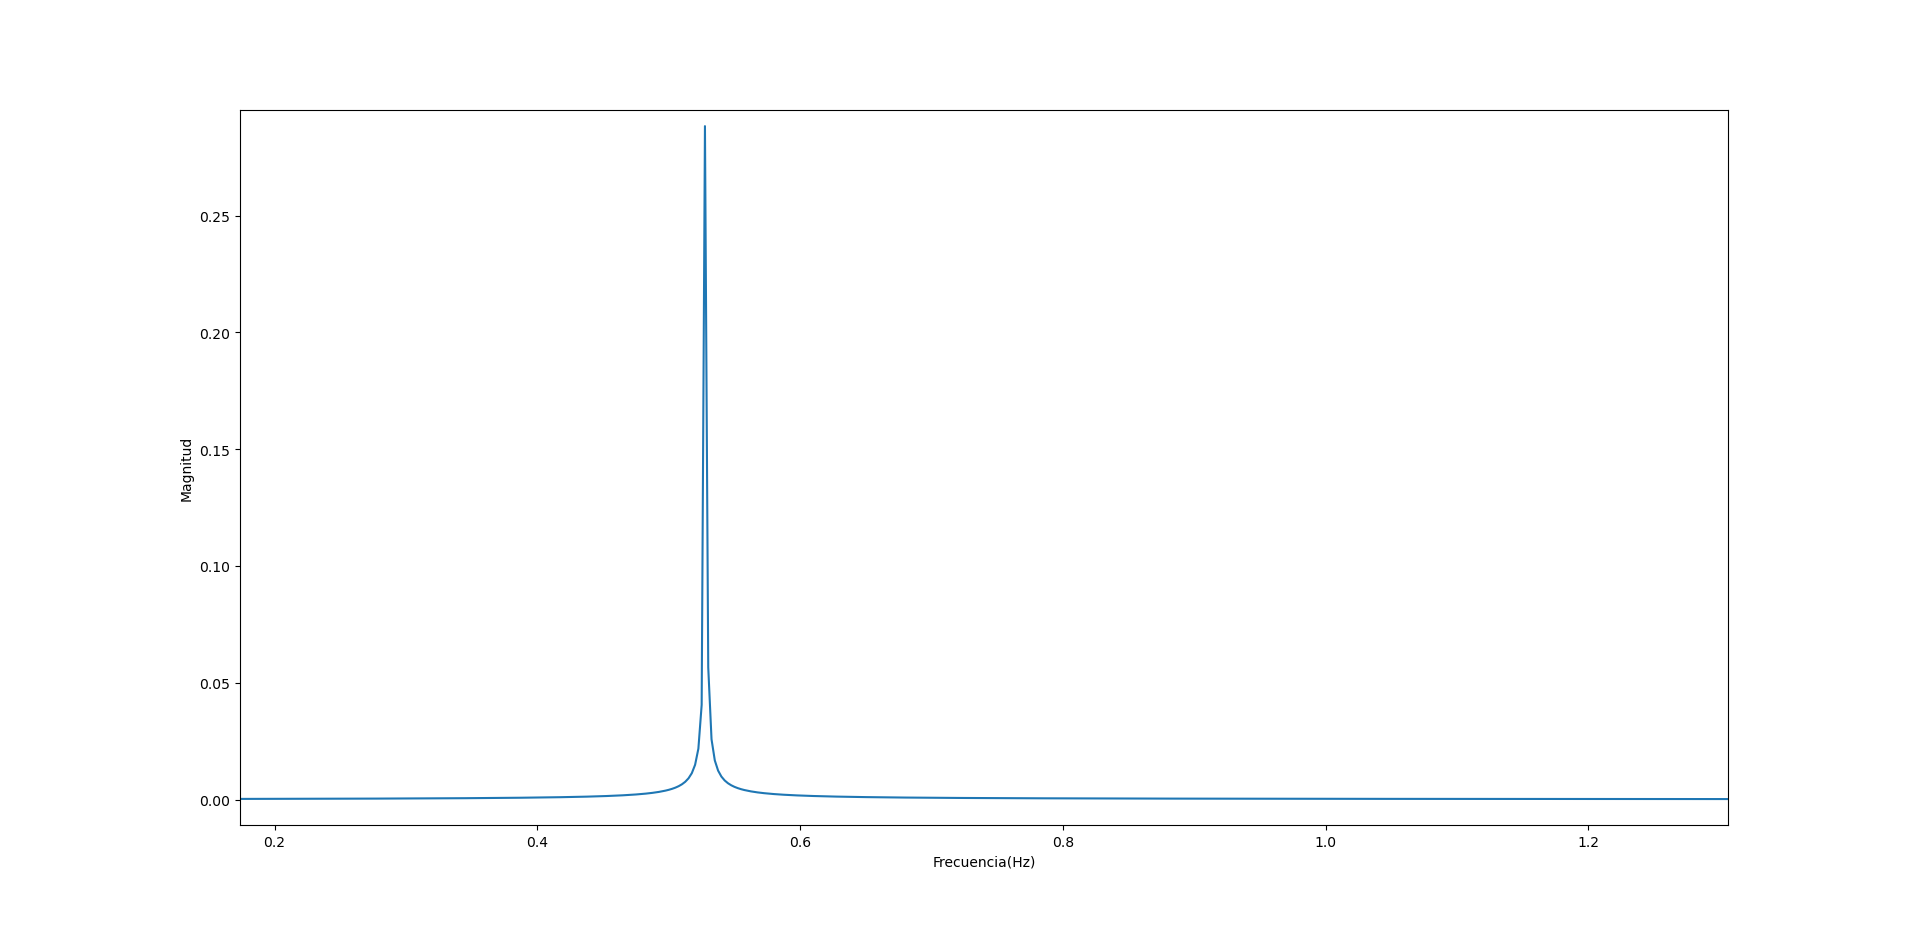
\includegraphics[width=0.8\textwidth]{antisimetrico_fourier}
\caption{Transformada de Fourier modo antisimétrico}
\label{fig:3}
\end{figure}
Podemos comprobar observando la Transformada de Fourier que el sistema solo va a tener un modo de vibración, que en este caso va a venir dada por $\omega =\sqrt{\frac{k+2k'}{m}}$, por lo que en este caso si modificamos $k'$ si que va a variar el movimiento del sistema, aumentando su frecuencia si aumentamos esta y disminuyendo al hacer lo contrario.
\section{Osciladores acoplados con gravedad}
Para terminar vamos a ver que ocurre si añadimos gravedad al sistema. Para ello vamos a colocar nuestro sistema en vertical y ver cómo afecta esta al movimiento. Consideraremos en este caso que ambas constantes elásticas son iguales y las demás condiciones iniciales serán iguales que en los casos estudiados en el apartado de dinámica del sistema.\newline\linebreak
Ahora la gravedad también ejercerá una fuerza sobre las masas, por lo que nuestras ecuaciones de movimiento del sistema cambiarán. Teniendo esto en cuenta y desarrollándolas llegamos a:

\begin{equation}
m(\ddot{x_1}-g)+(k+k')x_1 -k'x_2 = 0\label{ec.:1}
\end{equation}
\begin{equation}
m(\ddot{x_2}-g)+(k+k')x_2 -k'x_1  = 0\label{ec.:2}
\end{equation}
,siendo $g = 9.81\hspace{0.1cm}m/s^2$ la constante de gravedad.\newline\linebreak
Además, la fuerza de la gravedad, al ser una fuerza conservativa lleva una energía potencial asociada a ella de la forma $U_g =-mgy$ que se ejercerá sobre cada masa, por lo que tendremos que añadir esta energía a nuestro sistema.
\begin{figure}[H]
    \centering
    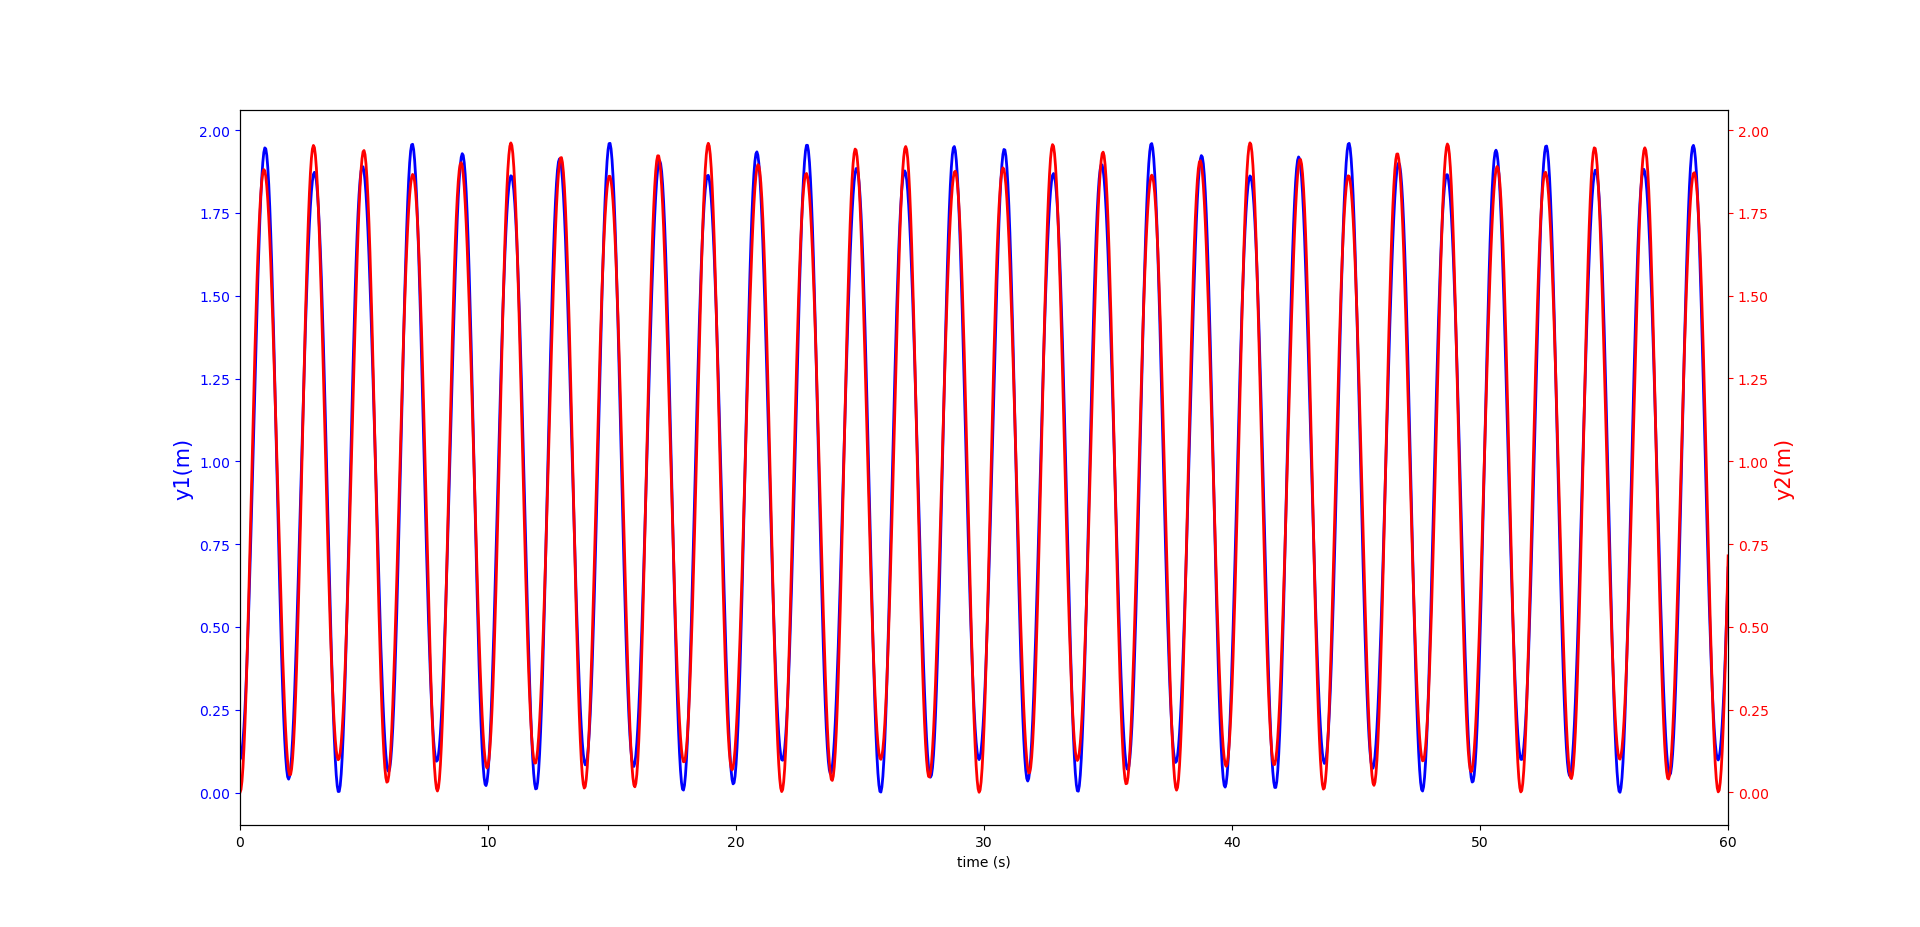
\includegraphics[width=1.0\textwidth]{gravedad}
\caption{Movimiento del sistema con gravedad}
\label{fig:10}
\end{figure}
Al representar el movimiento de cada una de las masas vemos que se mueven prácticamente en fase pero no llega a ser así debido a la fuerza que ejerce el muelle que une las dos masas.
Esto también lo podemos ver gracias a la Transformada de Fourier (Figura \ref{fig:f20}) donde vemos las frecuencias propias del sistema. En este caso vemos que tenemos dos frecuencias propias como es de esperar pero vemos que una de las dos es mucho más pequeña, y como el movimiento de las masas viene dado por la combinación lineal de ambas frecuencias por esto se da el movimiento que observamos.
\begin{figure}[H]
    \centering
    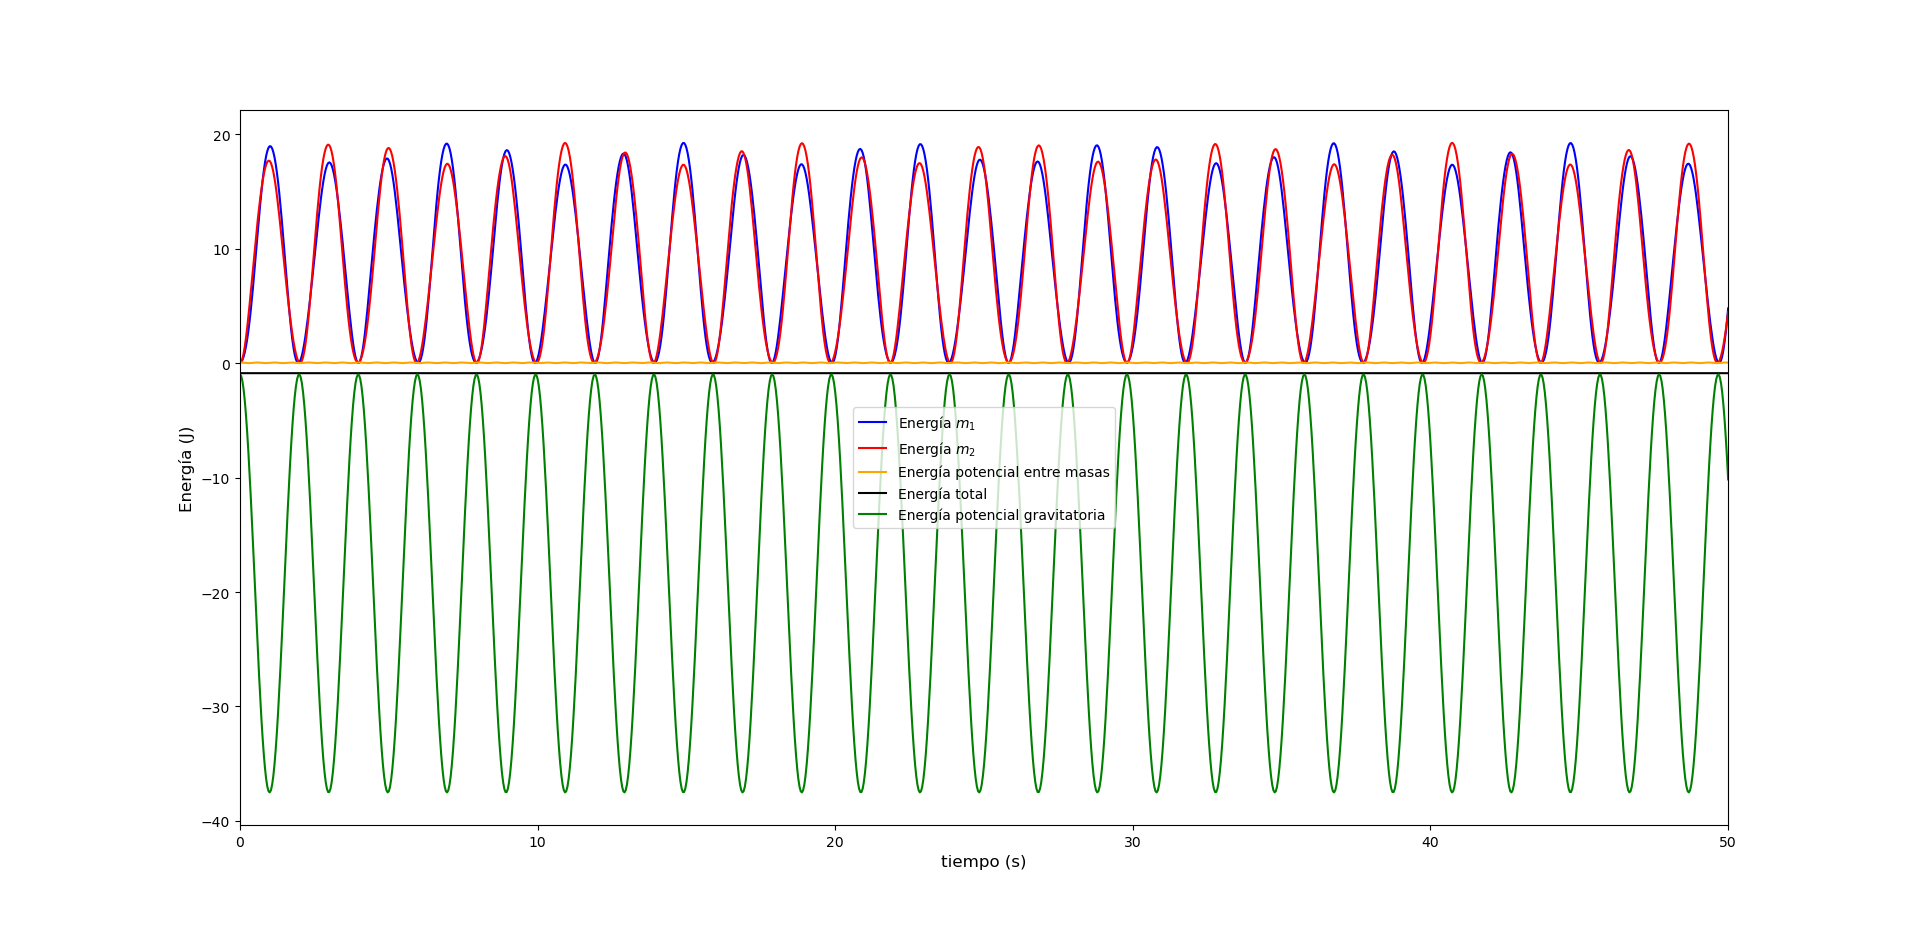
\includegraphics[width=1.0\textwidth]{gravedad_energias}
\caption{Energías del sistema con gravedad}
\label{fig:f}
\end{figure}
Si observamos las energías del sistema vemos que en este caso también tenemos la energía potencial que genera la fuerza gravitatoria. También vemos que la energía potencial del muelle que une las dos masas es prácticamente nula. Esto se debe a que la distancia entre las masas es aproximadamente de $0.1\hspace{0.1cm}m$ en todo momento. Además podemos ver que debido a la energía potencial gravitatoria en este caso la energía total del sistema va a ser negativa.
\begin{figure}[H]
    \centering
    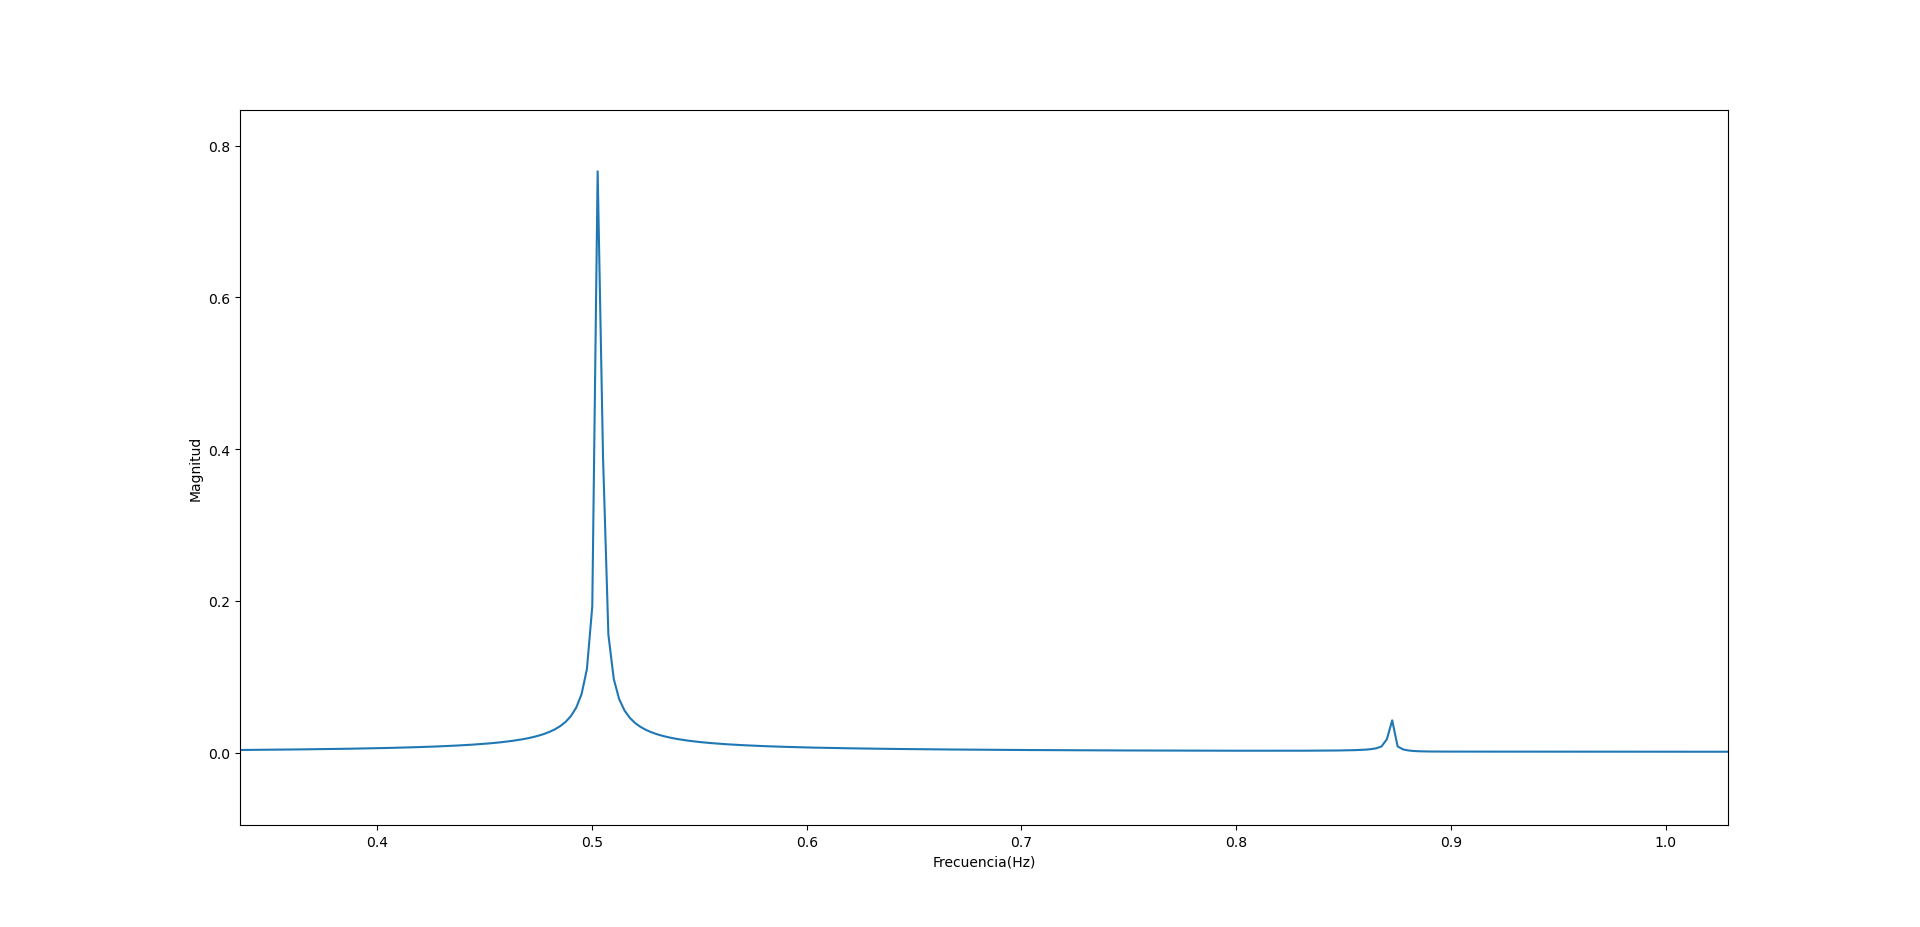
\includegraphics[width=1.0\textwidth]{gravedad_fourier}
\caption{Transformada de Fourier del sistema con gravedad}
\label{fig:f20}
\end{figure}
\section{Conclusiones}
En esta práctica hemos podido ver el comportamiento de un oscilador acoplado compuesto por 2 masas de igual magnitud ligadas por un muelle. Hemos comprobado que el movimiento cambia si modificamos la constante del muelle que une las masas debido a la fuerza que ejerce este, siendo la ligadura más fuerte cuando esta es más grande.\newline\linebreak
También vemos que las frecuencias propias del sistema van a cambiar al variar las constantes ya que dependen directamente de estas y que podemos describir el movimiento de las masas como combinación lineal de estas frecuencias.\newline\linebreak
Además, hemos podido ver que se cumple el principio de conservación de la energía mecánica en cualquier caso ya que todas las fuerzas que hemos considerado en el sistema son conservativas.\newline\linebreak
Por último, hemos podido estudiar los modos normales de vibración donde hemos visto la dependencia del movimiento en función de las condiciones iniciales y también hemos visto el comportamiento del sistema cuando añadimos la gravedad.
\section{Bibliografía}
\begin{thebibliography}{99}
\bibitem{mov}Guión de Prácticas osciladores acoplados
\bibitem{mov}\url{http://www.sc.ehu.es/sbweb/fisica/oscilaciones/acoplados/acoplados.html}

\end{thebibliography}
\end{document}